\chapter{Estymacja przykładowych modeli}
\label{ch:analiza}

W niniejszym rozdziale przedstawiono wyniki modelowania cen energii za pomocą czterech modeli: regresji liniowej, regresji Ridge, Propheta oraz MLP. Analiza została podzielona na dwa podrozdziały, odpowiadające okresom stabilnemu i niestabilnemu. Zbiór danych został poddany testom w celu oceny skuteczności. W celu uzyskania najlepszych wyników dla modeli przeprowadzono strojenie hiperparametrów.

\section{Okres stabilny}
\label{sec:okres_stabilny}

\subsubsection{Regresja liniowa i Ridge}

Przeanalizowano modele regresji liniowej oraz regresji Ridge na danych z okresu stabilnego. Modele trenowano na danych z lat 2016--2018, a testowano na danych z 2019 roku.

Wyniki dla pełnego zbioru o 60 parametrach wejściowych przedstawiono w tabeli~\ref{tab:linear_ridge_results_full}. Regresja Ridge osiągnęła lepsze wyniki niż regresja liniowa, co jest widoczne w tabeli poniżej na podstawie przedstawionych wcześniej metryk ~\ref{sec:ocena_jakosci_prognoz}. Wynika to z powodu regularyzacji L2 zastosowanej w modelu Ridge. 

\begin{table}[H]
    \centering
    \caption{Wyniki regresji liniowej i grzebietowej dla pełnego zbioru danych w okresie stabilnym (2019).}
    \label{tab:linear_ridge_results_full}
    \begin{tabular}{|l|ccccc|}
        \hline
        \textbf{Model} & \textbf{MAE} & \textbf{RMSE} & \textbf{MAPE (\%)} & \textbf{sMAPE (\%)} & \textbf{\(R^2\)} \\
        \hline
        Regresja liniowa & 15.18 & 19.79 & 7.25 & 7.16 & 0.8413 \\
        Regresja Ridge   & 15.09 & 19.64 & 7.19 & 7.09 & 0.8437 \\
        \hline
    \end{tabular}
\end{table}

Najlepsza wartość hiperparametru \(\alpha\) w regresji Ridge wyniosła 500.0. Wysoka wartość \(\alpha = 500.0\) sugeruje, że w pełnym zbiorze danych występuje istotna współliniowość między zmiennymi objaśniającymi. Potwierdza to również analiza macierzy korelacji ~\ref{fig:correlation_plot}.

Następnie przeprowadzono analizę skróconego zbioru danych opisanego w~\ref{sec:shortened_dataset}. Wyniki dla skróconego zbioru danych są przedstawione w tabeli~\ref{tab:linear_ridge_results_short}, wraz z różnicami w metrykach względem pełnego zbioru danych. Różnice w metrykach wskazują, że dodatkowe zmienne w pełnym zbiorze danych wnoszą informację, mimo niższego poziomu korelacji ze zmienną objaśnianą. Różnice metryk nie są bardzo duże (np. MAPE różni się o 0.16\% dla regresji Ridge), co może sugerować, że skrócony zbiór danych nadal zawiera najważniejsze zmienne objaśniające.

\begin{table}[h]
    \centering
    \caption{Wyniki regresji liniowej i Ridge dla skróconego zbioru danych w okresie stabilnym (2019) wraz z różnicami względem pełnego zbioru.}
    \label{tab:linear_ridge_results_short}
    \begin{tabular}{|l|ccccc|c|}
        \hline
        \textbf{Model} & \textbf{MAE} & \textbf{RMSE} & \textbf{MAPE (\%)} & \textbf{sMAPE (\%)} & \textbf{\(R^2\)} & \textbf{Różnica MAPE (\%)} \\
        \hline
        Regresja liniowa & 15.61 & 20.31 & 7.33 & 7.32 & 0.8328 & +0.08 \\
        Regresja Ridge   & 15.67 & 20.40 & 7.35 & 7.34 & 0.8314 & +0.16 \\
        \hline
    \end{tabular}
\end{table}

W celu potencjalnego polepszenia wyników zastosowano logarytmizację zmiennej wyjściowej (\texttt{fixing\_i\_price}), co miało na celu zmniejszenie skośności rozkładu cen i poprawę dopasowania modelu. Wyniki z logarytmizacją przedstawiono w tabeli~\ref{tab:linear_ridge_results_log}.

\begin{table}[h]
    \centering
    \caption{Wyniki regresji liniowej i Ridge z logarytmizacją dla okresu stabilnego (2019).}
    \label{tab:linear_ridge_results_log}
    \begin{tabular}{|l|ccccc|}
        \hline
        \textbf{Model i zbiór danych} & \textbf{MAE} & \textbf{RMSE} & \textbf{MAPE (\%)} & \textbf{sMAPE (\%)} & \textbf{\(R^2\)} \\
        \hline
        Regresja liniowa (pełny)   & 21.63 & 28.36 & 9.85 & 9.16 & 0.6736 \\
        Regresja Ridge (pełny)     & 19.99 & 26.06 & 9.21 & 8.65 & 0.7244 \\
        Regresja liniowa (skrócony) & 26.36 & 33.07 & 11.95 & 10.94 & 0.5563 \\
        Regresja Ridge (skrócony)   & 23.29 & 29.38 & 10.69 & 9.89 & 0.6498 \\
        \hline
    \end{tabular}
\end{table}

Logarytmizacja nie przyniosła spodziewanych korzyści i pogorszyła wyniki we wszystkich metrykach. Największe pogorszenie zaobserwowano dla skróconego zbioru danych, gdzie MAPE dla regresji liniowej wzrosło do 11.95\%, a \(R^2\) spadło do 0.5563. Przyczyną jest najprawdopodobniej fakt, że logarytmizacja wprowadziła niepotrzebne nieliniowości, które utrudniły dopasowanie modeli liniowych. Dodatkowo, odwrócenie transformacji logarytmicznej może amplifikować błędy predykcji, co wpłynęło na wzrost RMSE i MAE.

Regresja Ridge lepiej przewiduje ceny w porównaniu do regresji liniowej, co potwierdzają wyniki metryk. Poniżej umieszczam wykres rzeczywistych i przewidywanych wartości dla regresji Ridge w okresie stabilnym. Załączony został wykres z pierwszego kwartału 2019 roku, ponieważ wykres z całego 2019 nie jest czytelny z powodu dużej liczby punktów.

\begin{figure}[H]
    \centering
    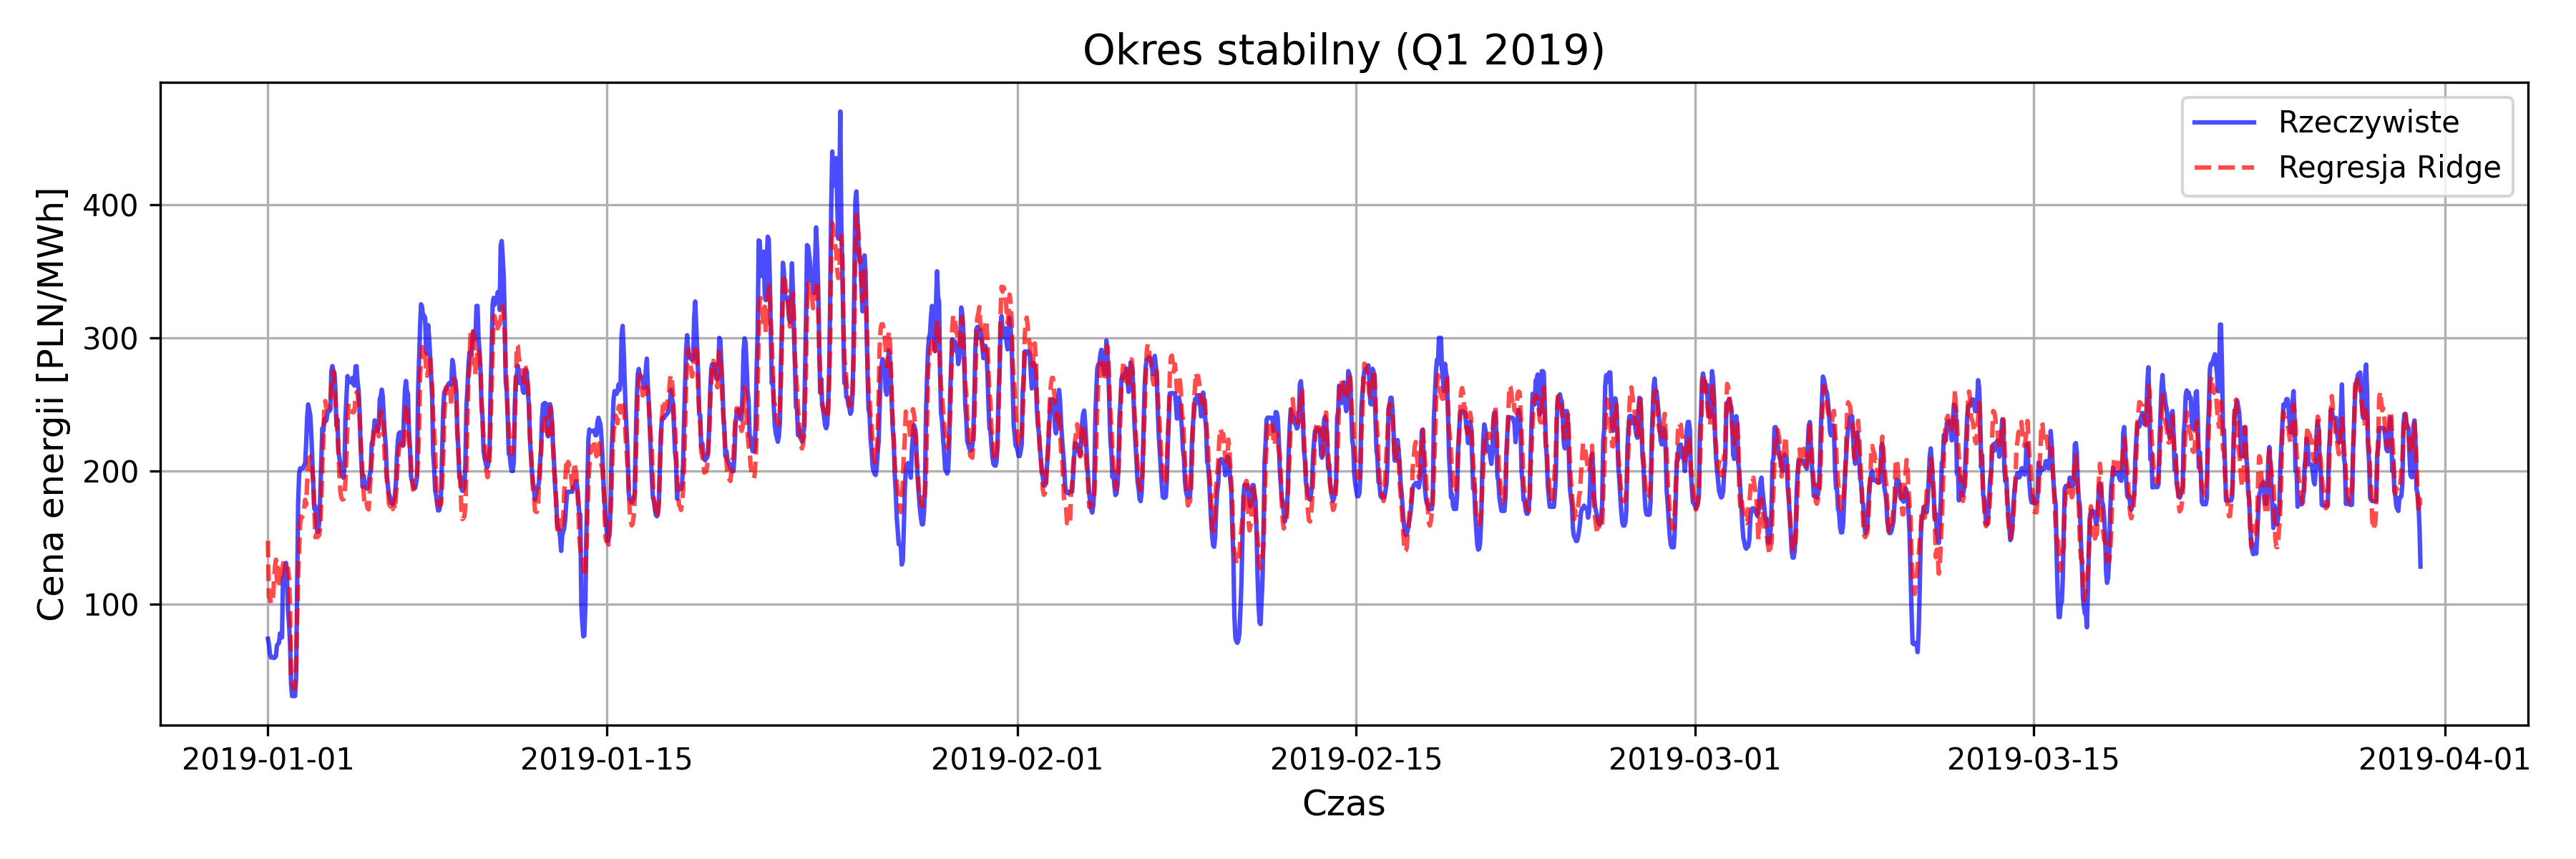
\includegraphics[width=1.0\textwidth]{../../plots/predicts/ridge_predictions_full_q1_2019.png}
    \caption{Porównanie rzeczywistych i przewidywanych wartości cen energii dla regresji Ridge w okresie stabilnym. Opracowanie własne.}
    \label{fig:ridge_predictions_full_stable_period}
\end{figure}

Widoczne na wykresie jest to, że model nie zawsze nadążą za dużymi skokami cen energii, prawdopodobnie z powodu ich nieliniowości. Z kolei w przypadku okresów mniejszych zmian i stabilniejszych cen, model oczekuje większej zmienności, co prowadzi do przeszacowania prognoz. Poniżej załączony jest wykres błędów dla regresji Ridge.

\begin{figure}[H]
    \centering
    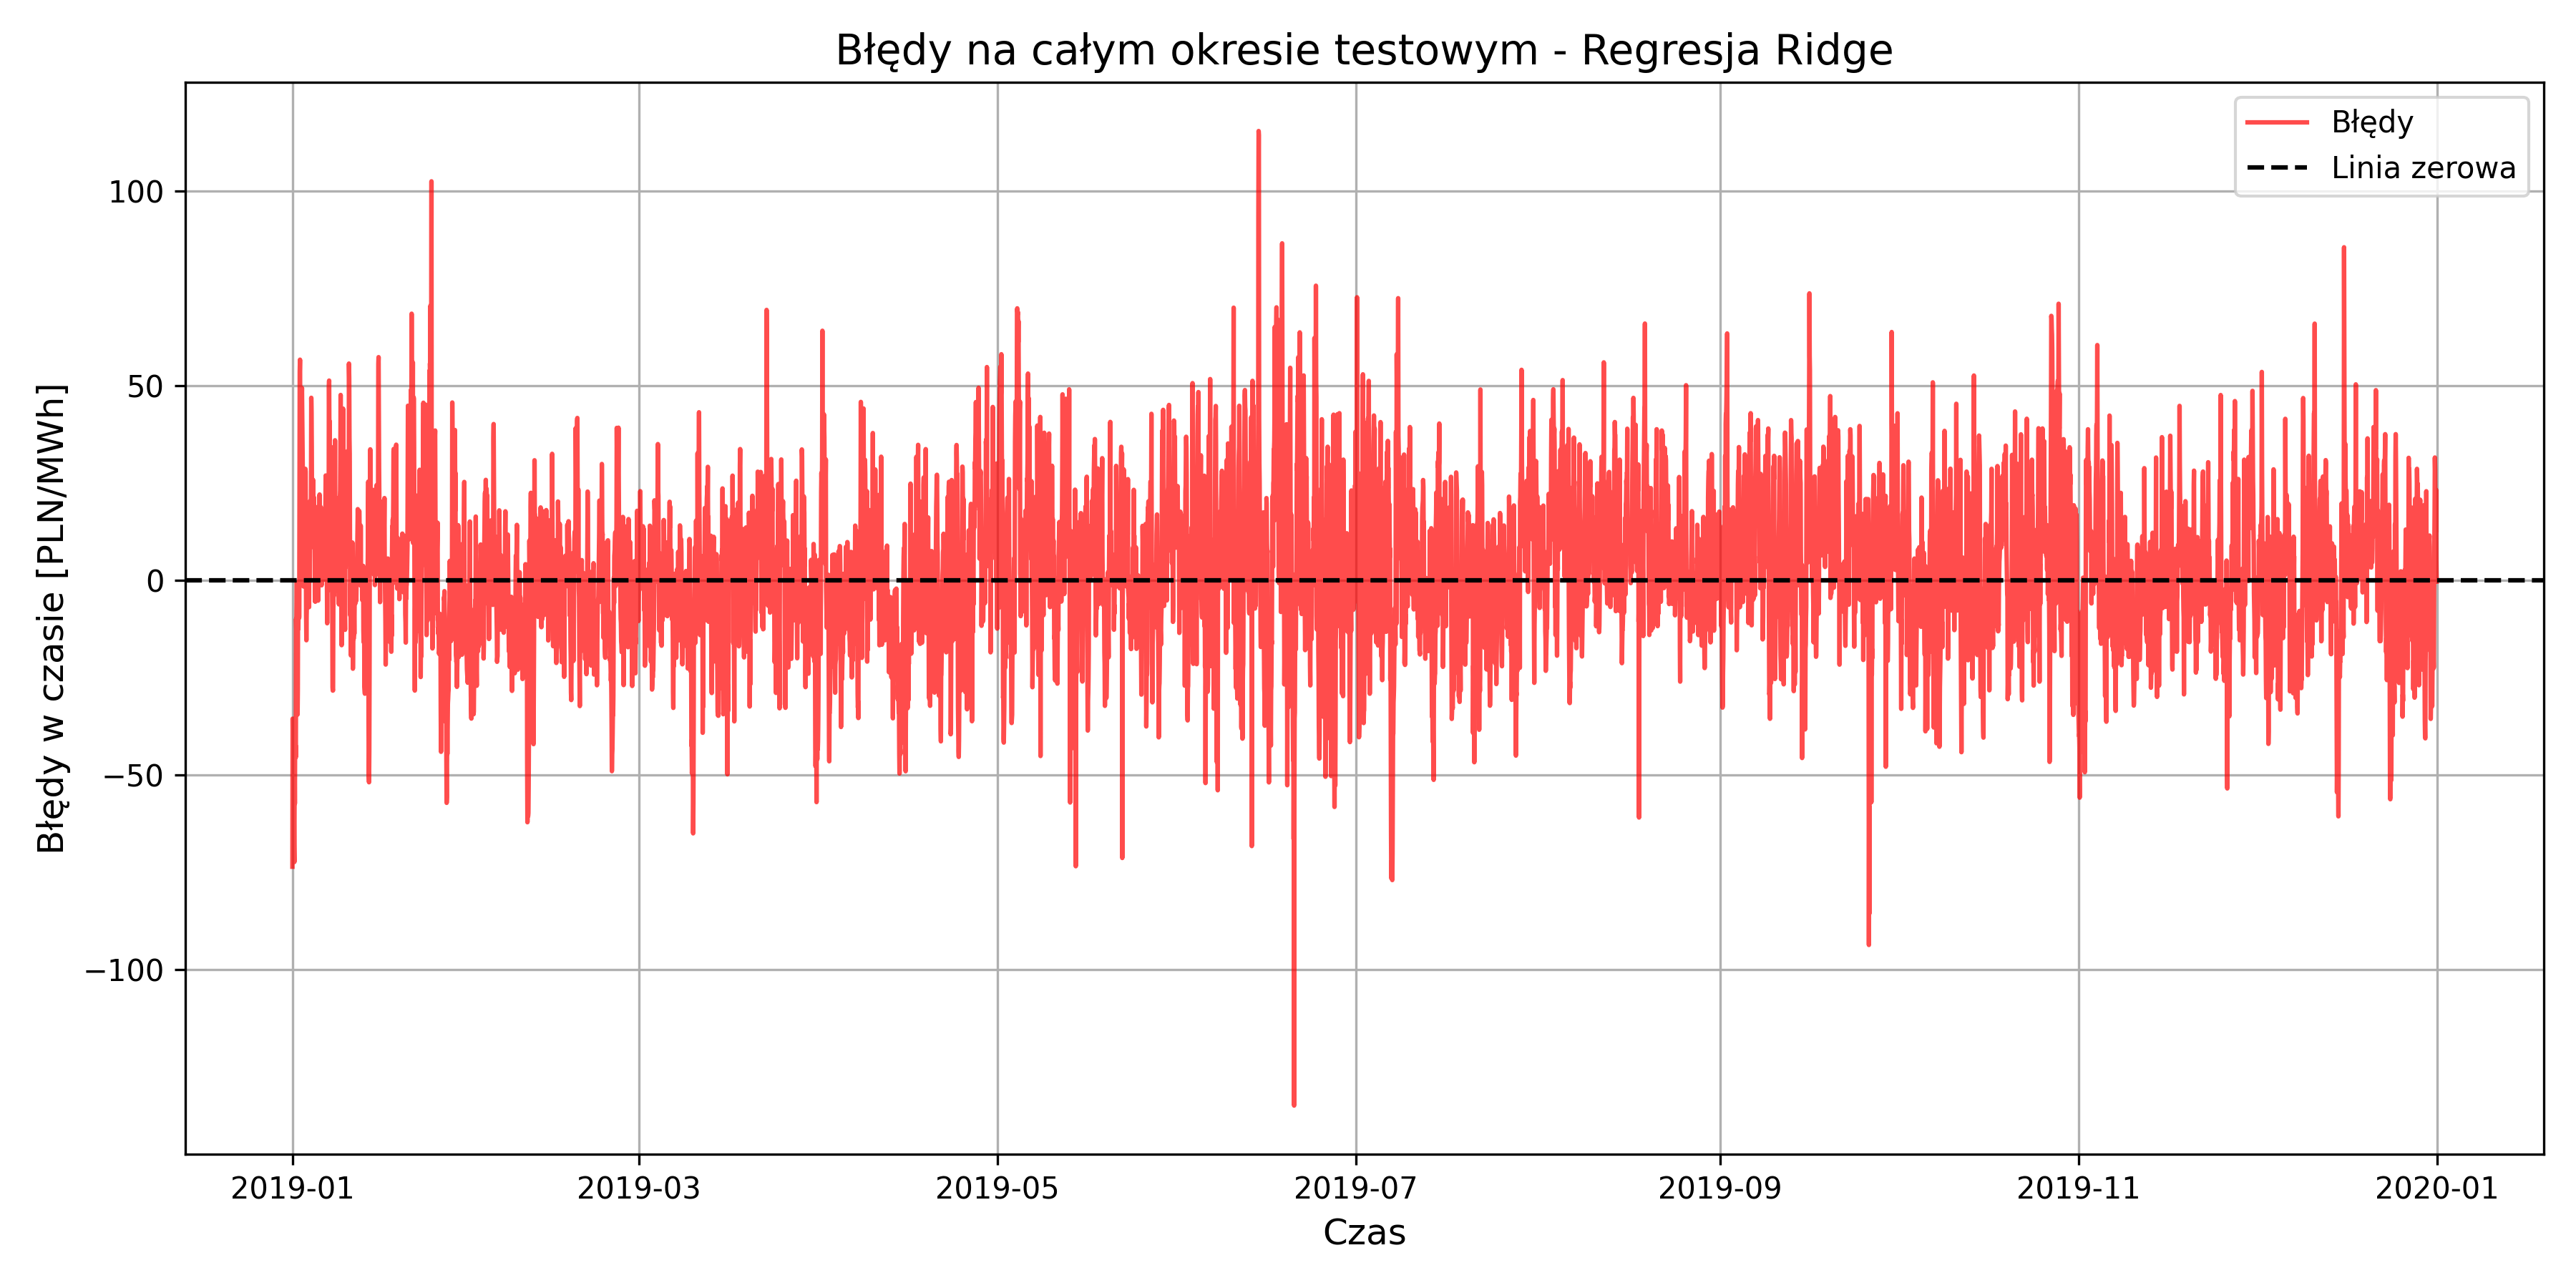
\includegraphics[width=1.0\textwidth]{../../plots/predicts/errors_over_time_Ridge_full_stable_period.png}
    \caption{Błędy prognoz dla regresji Ridge w okresie stabilnym. Opracowanie własne.}
    \label{fig:ridge_errors_full_stable_period}
\end{figure}

Błędy prognoz dla regresji Ridge w okresie stabilnym są rozproszone wokół zera, co sugeruje, że model dobrze radzi sobie z przewidywaniem cen energii elektrycznej. Wartości błędów przeważnie nie przekraczają 50 PLN/MWh. Widoczne są szczyty przekraczające 100 PLN/MWh, które mogą być wynikiem dużych skoków cen energii elektrycznej. Poniżej przedstawiony jest histogram reszt, żeby zobrazować rozkład błędów prognoz.

\begin{figure}[H]
    \centering
    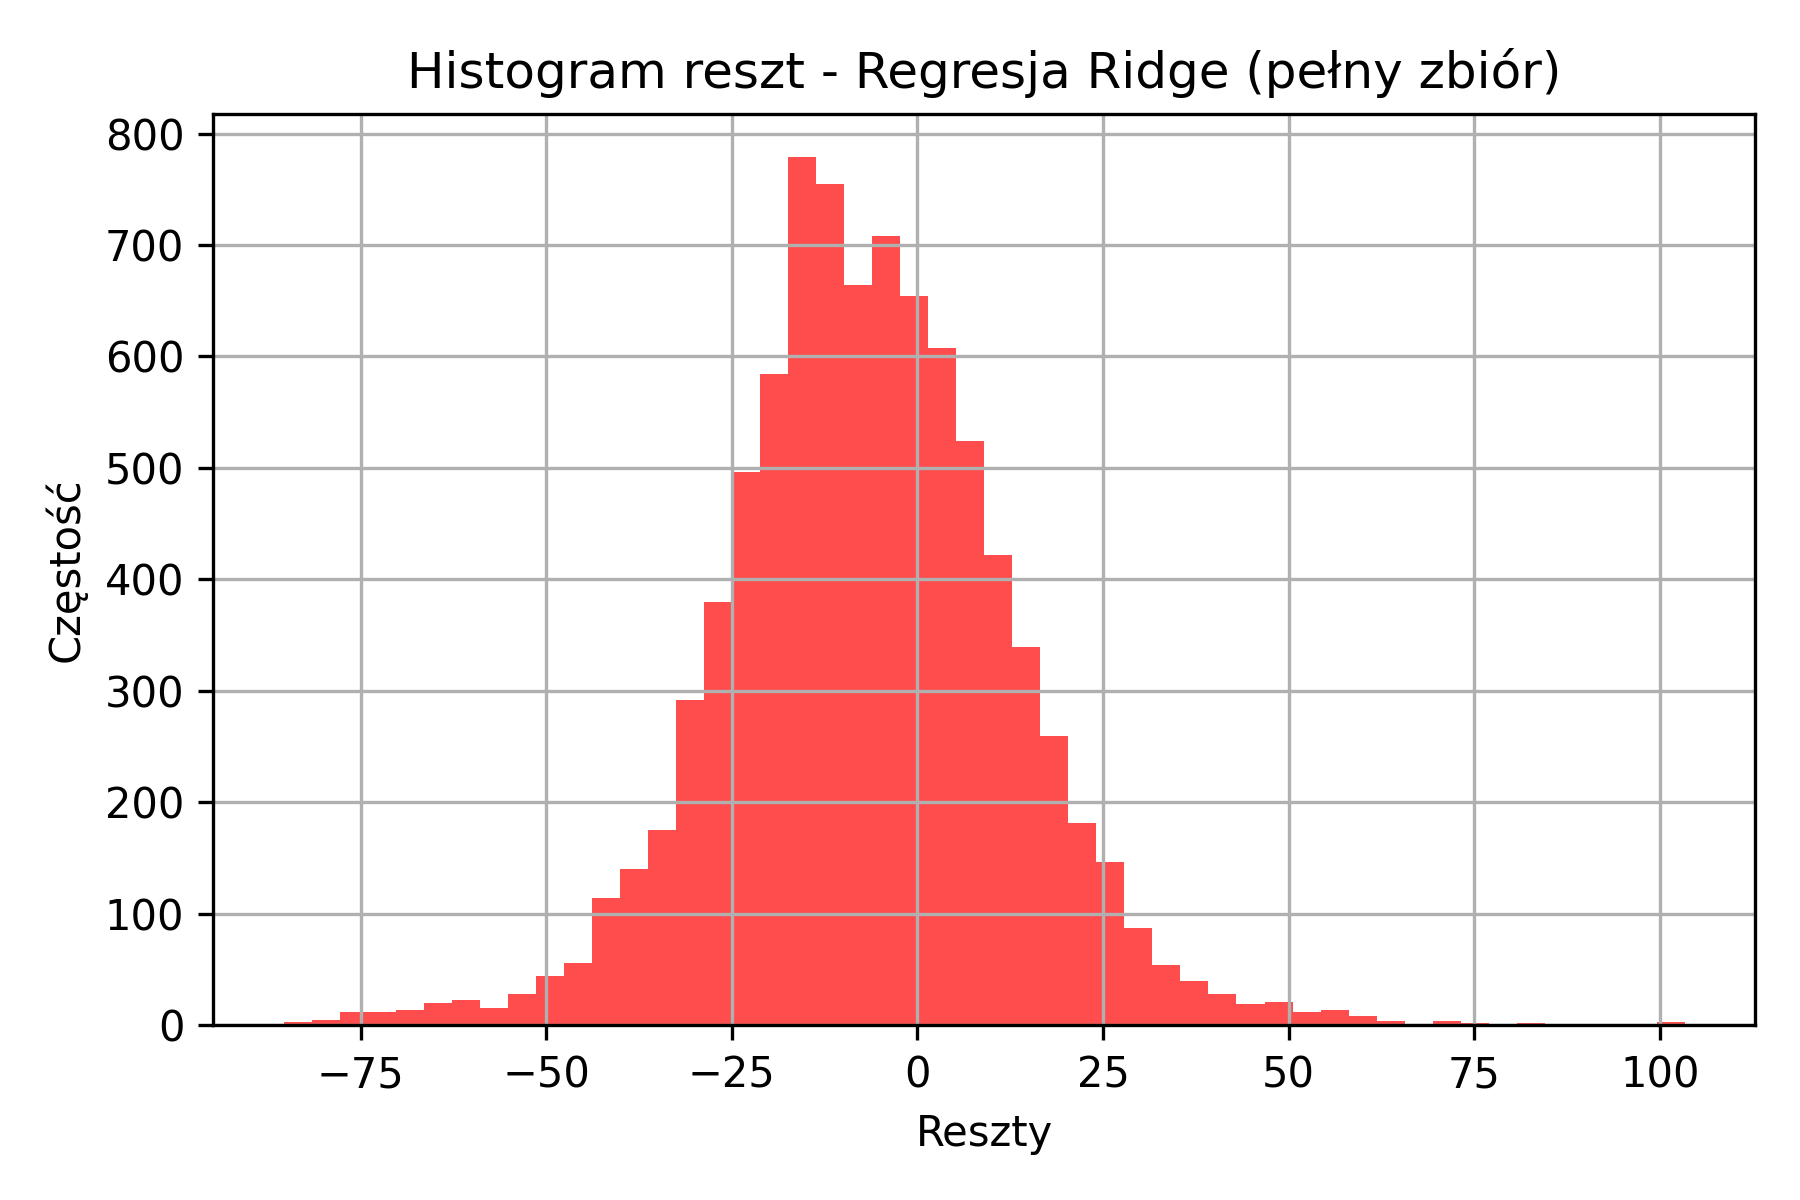
\includegraphics[width=1.0\textwidth]{../../plots/predicts/residuals_histogram_Ridge_full_stable_period.png}
    \caption{Histogram reszt dla regresji Ridge w okresie stabilnym. Opracowanie własne.}
    \label{fig:ridge_residuals_stable_period}
\end{figure}

Histogram posiada szczyt w okolicy zera i większość błędów skupia się w okolicy zera. Rozkład reszt jest zbliżony do normalnego bez istotnych odchyleń. Wartości reszt są rozproszone w okolicy zera, co sugeruje, że model dobrze radzi sobie z przewidywaniem cen energii elektrycznej w okresie stabilnym. Widoczne na wykresie ~\ref{fig:ridge_residuals_stable_period} szczyty dochodzące do 100 PLN/MWh nie są widoczne na histogramie, co sugeruje, że są to pojedyncze przypadki dużych błędów prognozowania. Wartości tych błędów nie mają wyraźnych wzorców czasowych ani sezonowych. Pojawienie się dużych błędów wynika z fluktuacji cen energii elektrycznej, wynikających z czynników nie wytłumaczalnych przez zbiór zmiennych objaśniających lub czynników zewnętrznych.

\subsubsection{Prophet}
Model Prophet został skonfigurowany z trybem addytywnym (\texttt{seasonality\_mode='additive'}), ponieważ wstępne testy wykazały, że tryb multiplikatywny (\texttt{seasonality\_mode='multiplicative'}) działa dużo gorzej w przypadku zebranych danych. Tryb multiplikatywny zakłada proporcjonalne skalowanie efektów sezonowych i trendów względem wartości zmiennej objaśnianej, co nie jest odpowiednie dla cen energii elektrycznej, gdzie efekty sezonowe (np. różnice między dniami roboczymi a weekendami) mają raczej charakter addytywny, a nie proporcjonalny.

Testowano różne kombinacje pozostałych hiperparametrów opisanych w rozdziale \ref{subsec:prophet}, aby znaleźć optymalne ustawienia. Najlepsze rezultaty uzyskano dla kombinacji (\texttt{changepoint\_prior\_scale=0.100}, \texttt{seasonality\_prior\_scale=20.0}, \texttt{holidays\_prior\_scale=0.1}), gdzie gdzie MAE wyniosło 15.60, RMSE 20.17, MAPE 7.42\%, a sMAPE 7.33\%. Kombinacja ta charakteryzuje się umiarkowaną elastycznością trendu (\texttt{changepoint\_prior\_scale=0.100}), co pozwala modelowi wychwytywać zmiany w cenach energii (np. stopniowe wzrosty), oraz wysoką elastycznością sezonowości (\texttt{seasonality\_prior\_scale=20.0}), co dobrze oddaje zmienne wzorce dzienne i tygodniowe. Niski wpływ świąt (\texttt{holidays\_prior\_scale=0.1}) sugeruje, że polskie święta mają ograniczony wpływ na ceny energii w tym okresie. Pełne wyniki dla pełnego zbioru danych przedstawiono w tabeli~\ref{tab:prophet_results_combined_stable}.

\begin{table}[H]
    \centering
    \caption{Wyniki modelu Prophet dla pełnego i skróconego zbioru danych w okresie stabilnym (2019).}
    \label{tab:prophet_results_combined_stable}
    \begin{tabular}{|l|ccccc|}
        \hline
        \textbf{Zbiór danych} & \textbf{MAE} & \textbf{RMSE} & \textbf{MAPE (\%)} & \textbf{sMAPE (\%)} & \textbf{\(R^2\)} \\
        \hline
        Pełny     & 15.60 & 20.17 & 7.42 & 7.33 & 0.835011 \\
        Skrócony  & 17.75 & 22.85 & 8.17 & 8.32 & 0.788273 \\
        \hline
    \end{tabular}
\end{table}

Pełny zbiór danych znowu osiągnął lepsze wyniki od zbioru skróconego. Różnice są większe, niż w przypadku regresji liniowej i Ridge, co sugeruje, że dodatkowe zmienne w pełnym zbiorze danych mają większy wpływ na prognozy modelu Prophet.

Ponizej przedstawiam wykresy rzeczywistych i przewidywanych wartości dla modelu Prophet dla pierwszego kwartału 2019 roku. Wykres jest bardzo podobny do wykresu \ref{fig:ridge_predictions_full_stable_period} dla regresji Ridge.

\begin{figure}[H]
    \centering
    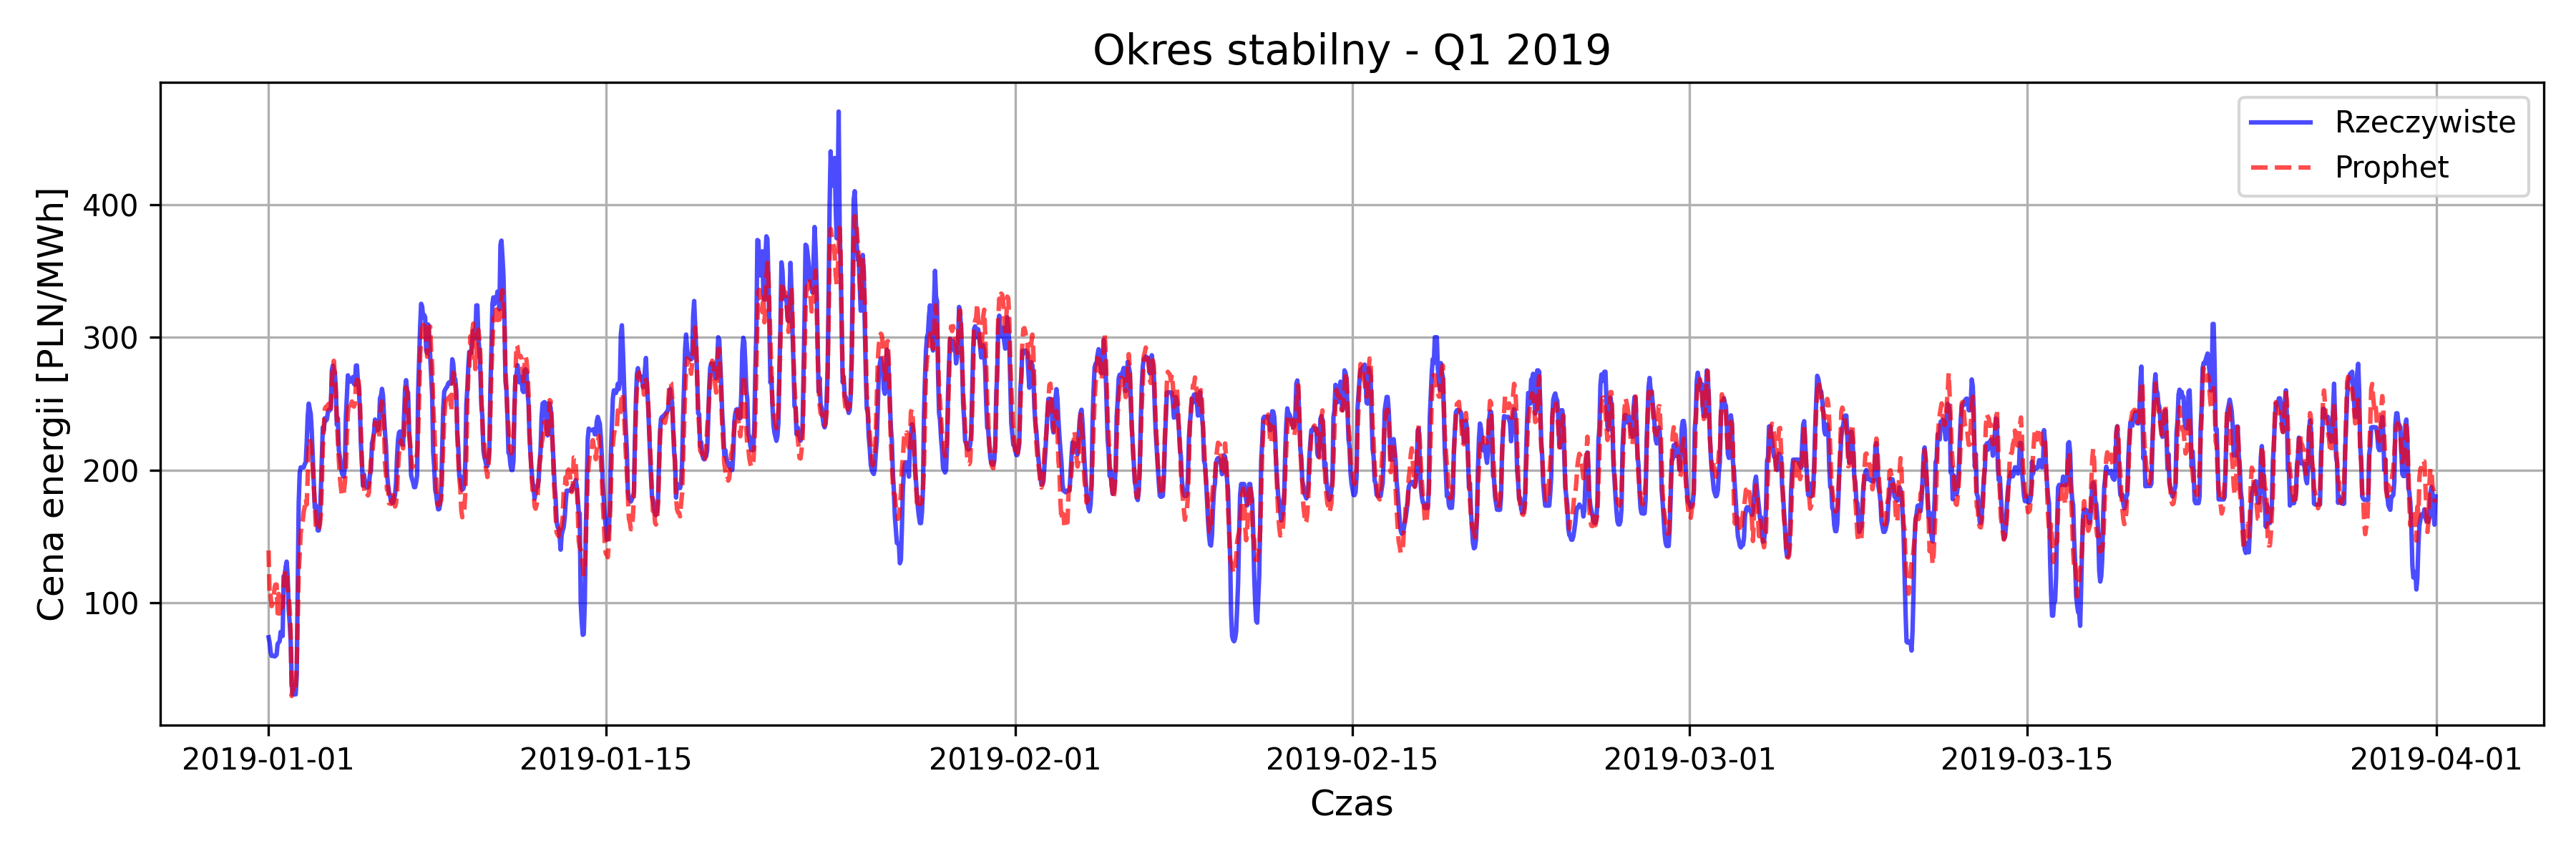
\includegraphics[width=1.0\textwidth]{../../plots/predicts/Prophet_predictions_stable_Q1.png}
    \caption{Porównanie rzeczywistych i przewidywanych wartości cen energii dla modelu Prophet w okresie stabilnym. Opracowane własne}
    \label{fig:prophet_predictions_stable_period}
\end{figure}

Wykres błędów prognoz dla modelu Prophet w okresie stabilnym jest również podobny do wykresu regresji Ridge~\ref{fig:ridge_errors_full_stable_period}.

\begin{figure}[H]
    \centering
    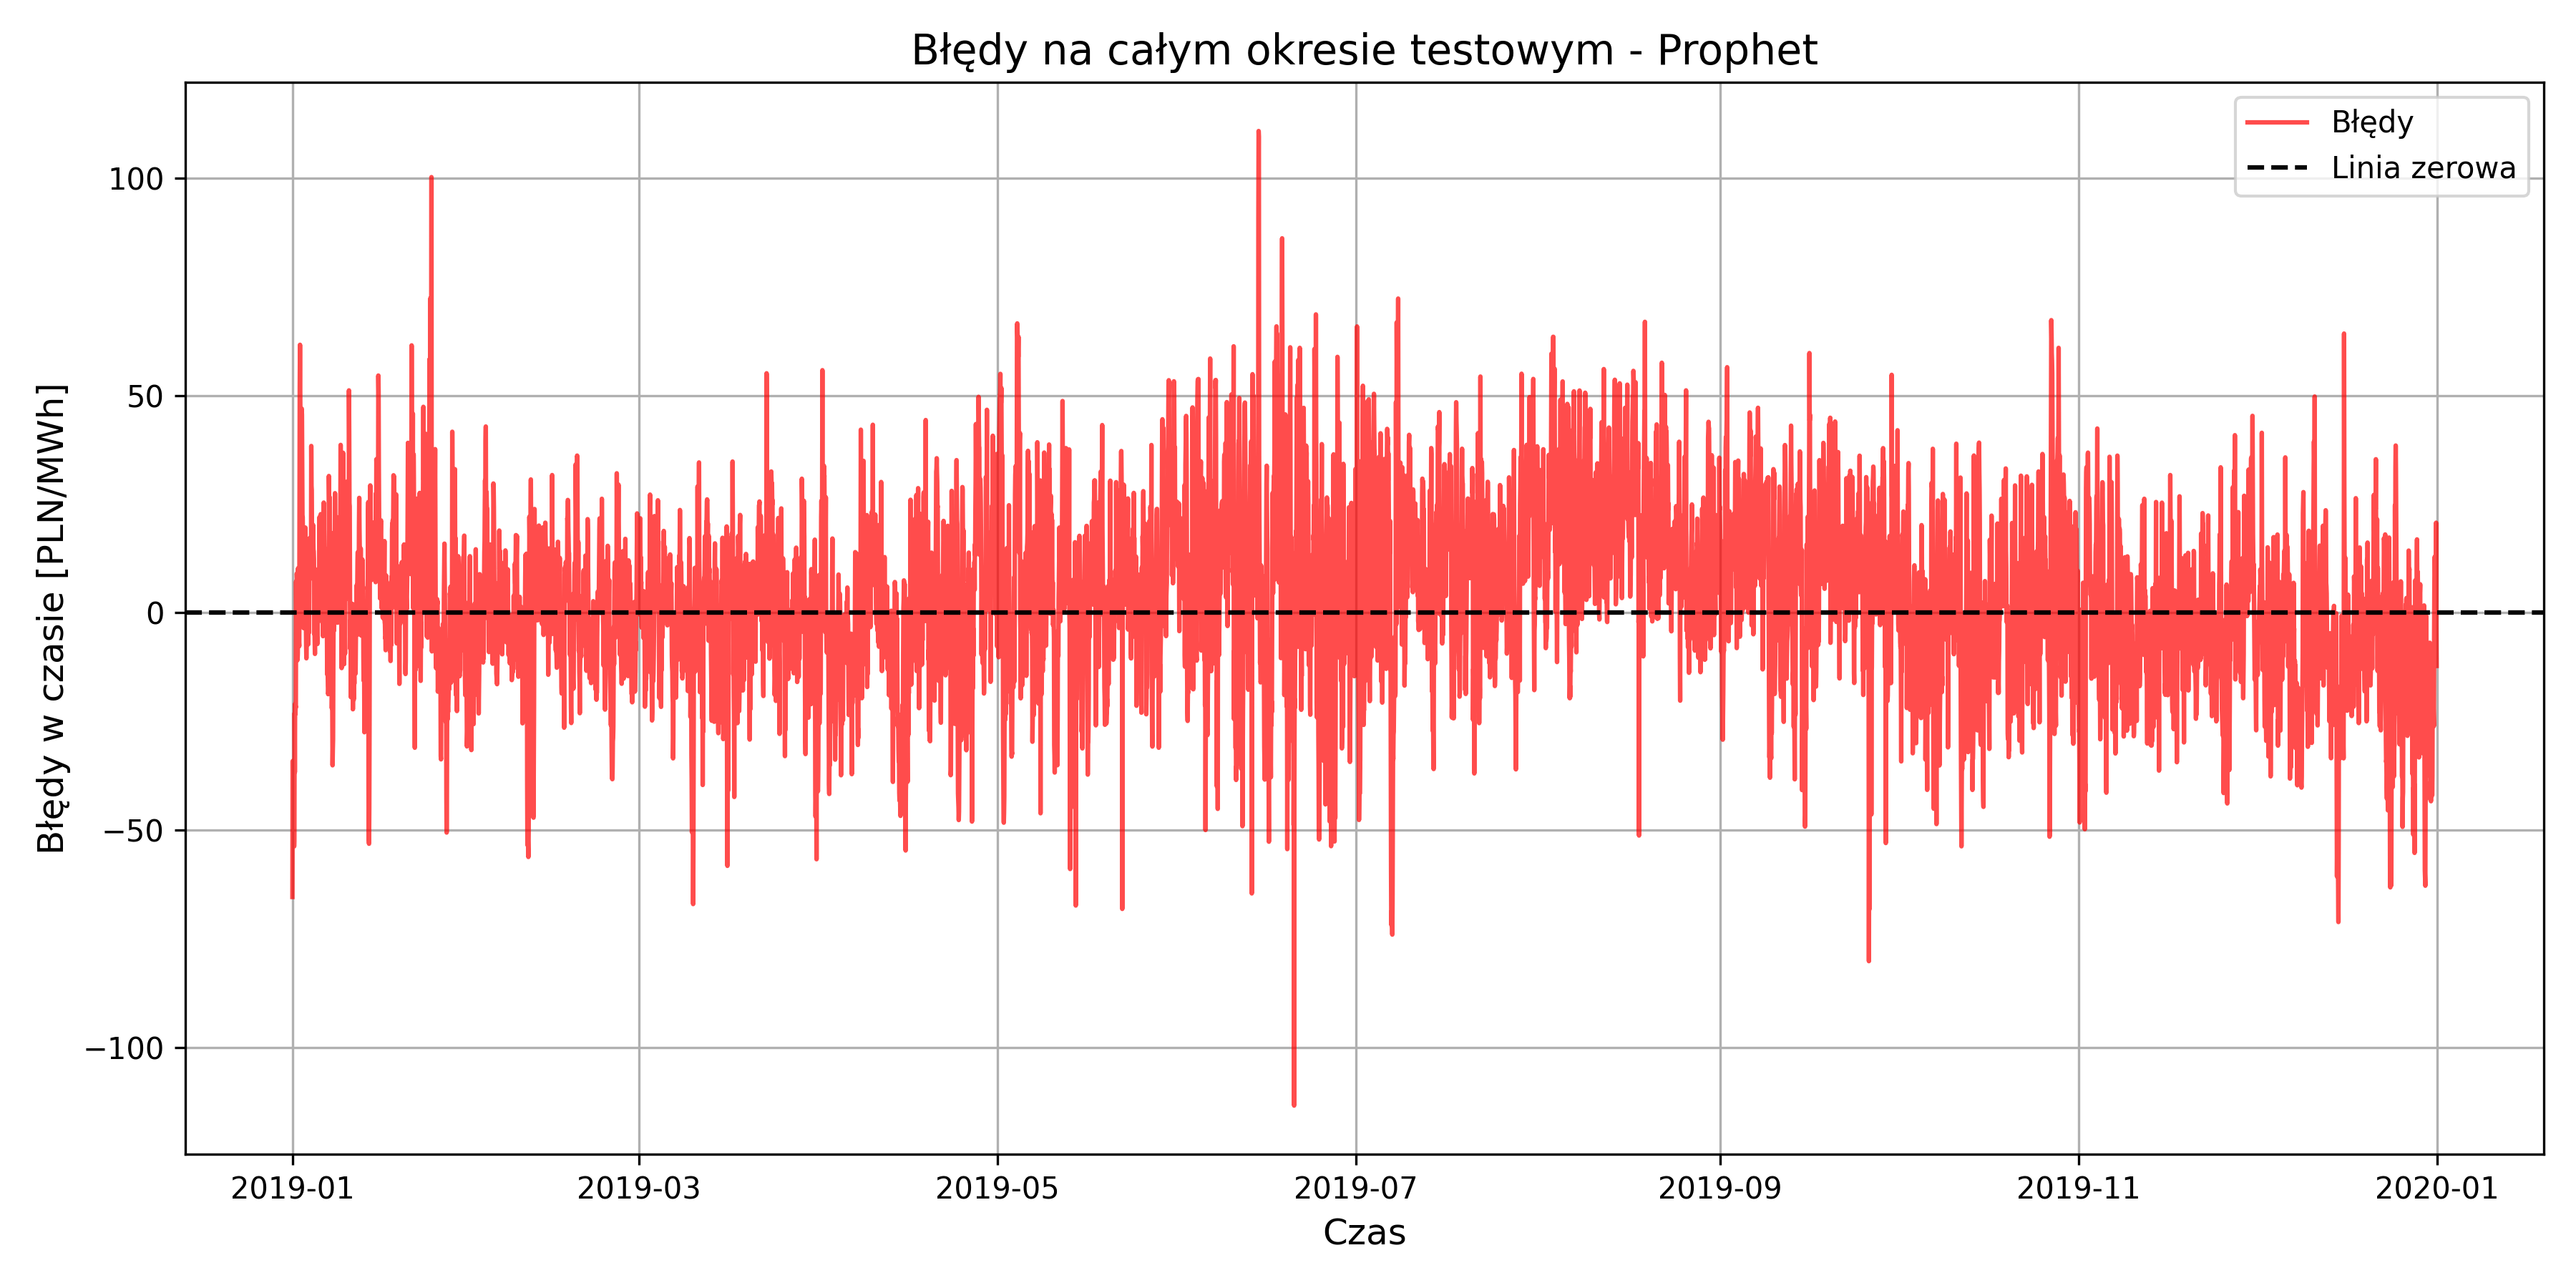
\includegraphics[width=1.0\textwidth]{../../plots/predicts/errors_over_time_Prophet_full_stable_period.png}
    \caption{Błędy prognoz dla modelu Prophet w okresie stabilnym.}
    \label{fig:prophet_errors_full_stable_period}
\end{figure}

Histogram reszt dla modelu Prophet wykazuje podobieństwo do histogramu reszt dla regresji Ridge~\ref{fig:ridge_residuals_stable_period}, ale lepiej wyjaśnia drobne różnice. Ma niższy szczyt w okolicy zera, ale łagodniejsze zejście w kierunku wartości skrajnych.

\begin{figure}[H]
    \centering
    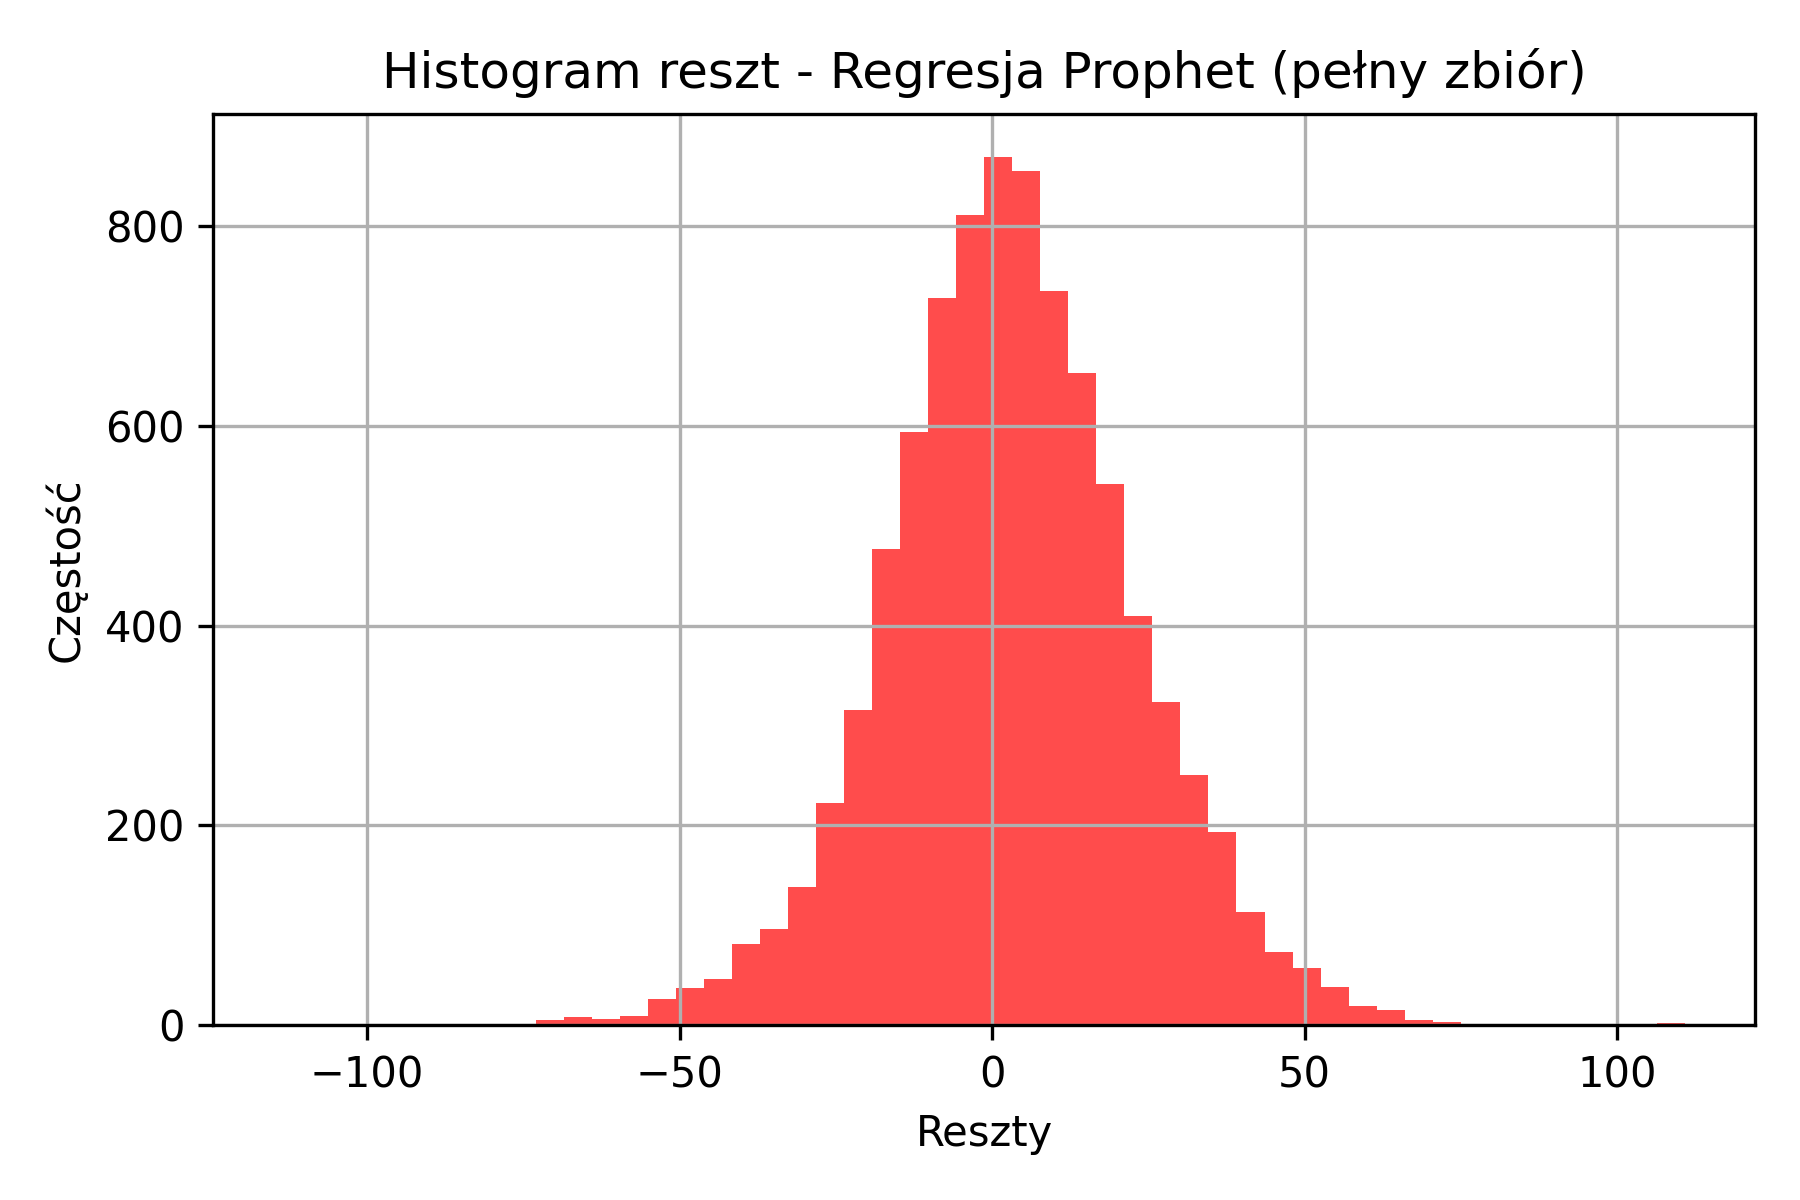
\includegraphics[width=1.0\textwidth]{../../plots/predicts/residuals_histogram_Prophet_full_stable_period_comb_1.png}
    \caption{Histogram reszt dla modelu Prophet w okresie stabilnym. Opracowanie własne.}
    \label{fig:prophet_residuals_stable}
\end{figure}

Największe błędy prognoz występujące w obu modelach są podobne. Największym wspólnym błędem prognoz dla modeli regresji Ridge oraz Prophet jest przeszacowanie ceny energii elektrycznej w dniu 10 Marca o godzinie 5 rano, gdzie rzeczywista cena wynosi 64 PLN/MWh, gdzie prognozy wynoszą 129 PLN/MWh oraz 131 PLN/MWh dla modelu Ridge i Prophet. Prawdopodobnie zmienne objaśniające sygnalizują wzrost cen, która nie miała miejsca, co prowadzi do przeszacowania prognoz.

Analizując wyniki modelu Prophet w odniesieniu do wyników regresji liniowej i grzbietowej, można stwierdzić, że model Prophet osiąga porównywalne wyniki. Wynik MAPE jest o 0.23\% wyższy od regresji Ridge, co sugeruje, że model Prophet nie jest w stanie przewidzieć cen energii elektrycznej lepiej. Natomiast czas wykonania programu w języku programowania \texttt{Python} dla modelu Prophet wynosił ponad 40 sekund, gdzie czas wykonania dla regresji Ridge wynosił 5. W kontekście analizy zebranego zbioru danych, należy zauważyć, że model Prophet nie przynosi żadnych korzyści w porównaniu do regresji Ridge lub liniowej w przypadku prognozowania w okresie stabilnym.

\subsubsection{MLP}

W ramach badania skuteczności modelu MLP w okresie stabilnym, obejmującym rok 2019, przetestowano różne konfiguracje sieci neuronowych. Najlepsze wyniki uzyskano dla architektury składającej się z pięciu warstw ukrytych, o strukturze z odpowiednio 64, 64, 32, 16 , 8 neuronami w kolejnych warstwach. Model został zaprojektowany w sposób sekwencyjny, gdzie każda warstwa ukryta korzystała z funkcji aktywacji ReLU, a dodatkowo zastosowano regularyzację L2 z parametrem 0,1, aby zapobiec przeuczeniu. Między warstwami dodano mechanizm Dropout z wartością 0,2, który losowo dezaktywuje część neuronów podczas treningu, co pomaga w uogólnianiu modelu. Ostatnia warstwa wyjściowa zawierała jeden neuron, odpowiadający za przewidywanie wartości ceny energii.

Model został skompilowany z użyciem optymalizatora Adam, skonfigurowanego z bardzo niską szybkością uczenia na poziomie 0,0001, co pozwoliło na stopniowe i stabilne dostosowywanie wag. Jako funkcję straty wybrano średni błąd kwadratowy (MSE), która dobrze mierzy różnice między przewidywaniami a rzeczywistymi wartościami. Trening modelu przeprowadzono na danych z lat 2016-2018, z maksymalną liczbą pięciuset epok i rozmiarem partii wynoszącym sto dwadzieścia osiem, co umożliwiło efektywne przetwarzanie danych w mniejszych porcjach.

W tabeli poniżej przedstawiam wyniki dla pełnego i skróconego zbiorów danych. 

\begin{table}[H]
    \centering
    \caption{Wyniki modelu MLP dla pełnego i skróconego zbioru danych w okresie stabilnym (2019).}
    \label{tab:mlp_results_combined_stable}
    \begin{tabular}{|l|cccccc|}
        \hline
        \textbf{Zbiór danych} & \textbf{MAE} & \textbf{RMSE} & \textbf{MAPE (\%)} & \textbf{sMAPE (\%)} & \textbf{\(R^2\)} \\
        \hline
        Pełny     & 17.09 & 22.75 & 8.43 & 7.87 & 0.79 \\
        Skrócony  & 34.55 & 53.58 & 14.87 & 13.56 & -0.16 \\
        \hline
    \end{tabular}
\end{table}

Uzyskane wyniki dla zbioru skróconego są znacznie gorsze niż dla zbioru pełnego, co sugeruje, że model MLP nie jest w stanie dobrze przewidzieć cen energii elektrycznej na podstawie ograniczonej liczby zmiennych objaśniających. Wartości MAPE są o ponad procent wyższe niż w przypadku regresji liniowej i Ridge, co sugeruje, że model MLP nie jest w stanie przewidzieć cen energii elektrycznej lepiej niż modele statystyczne. Inne zestawy parametrów lub architektury sieci neuronowej nie przyniosły lepszych wyników.

\begin{figure}[H]
    \centering
    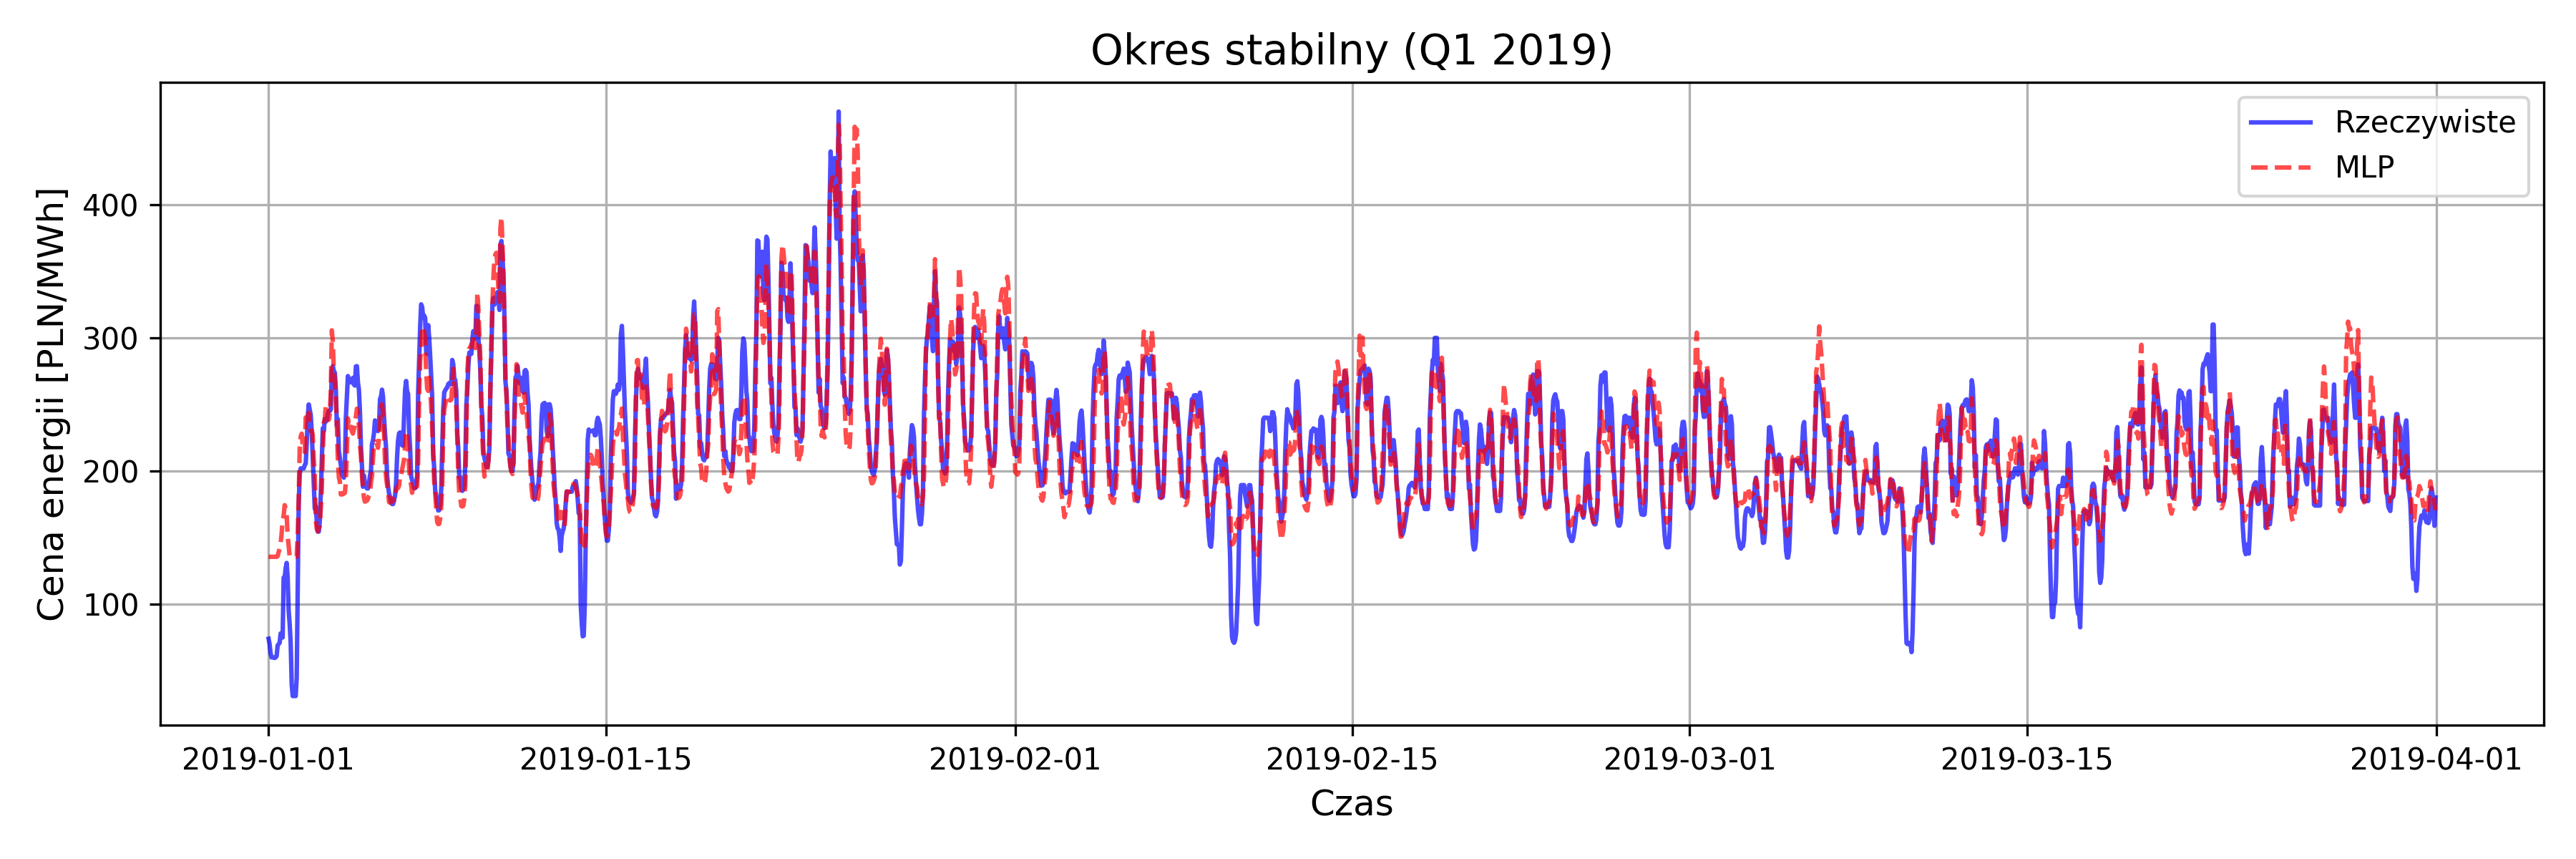
\includegraphics[width=1.0\textwidth]{../../plots/mlp1/mlp_predictions_full_stable_q1_(64, 64, 32, 16, 8).png}
    \caption{Porównanie rzeczywistych i przewidywanych wartości cen energii dla modelu MLP w okresie stabilnym. Opracowanie własne.}
    \label{fig:mlp_predictions_stable_period}
\end{figure}

Wykres~\ref{fig:mlp_predictions_stable_period} nieco różni się od analogicznych wykresów dla modeli statystycznych. Prognozy dobrze podążają za rzeczywistymi wartościami, ale widać, że model MLP ma tendencję do przeszacowywania cen energii elektrycznej w momentach wzrostów ceny. Model oczekuje na większe wzrosty, które nie następują.\newline
Poniżej przedstawione są wykresy błędów prognoz dla modelu MLP oraz histogram reszt dla okresu stabilnego. 

\begin{figure}[H]
    \centering
    \includegraphics[width=1.0\textwidth]{../../plots/mlp1/errors_over_time_(64, 64, 32, 16, 8)_Stabilny_2019_pełny.png}
    \caption{Błędy prognoz dla modelu MLP w okresie stabilnym. Opracowanie własne.}
    \label{fig:mlp_errors_stable_period}
\end{figure}

\begin{figure}[H]
    \centering
    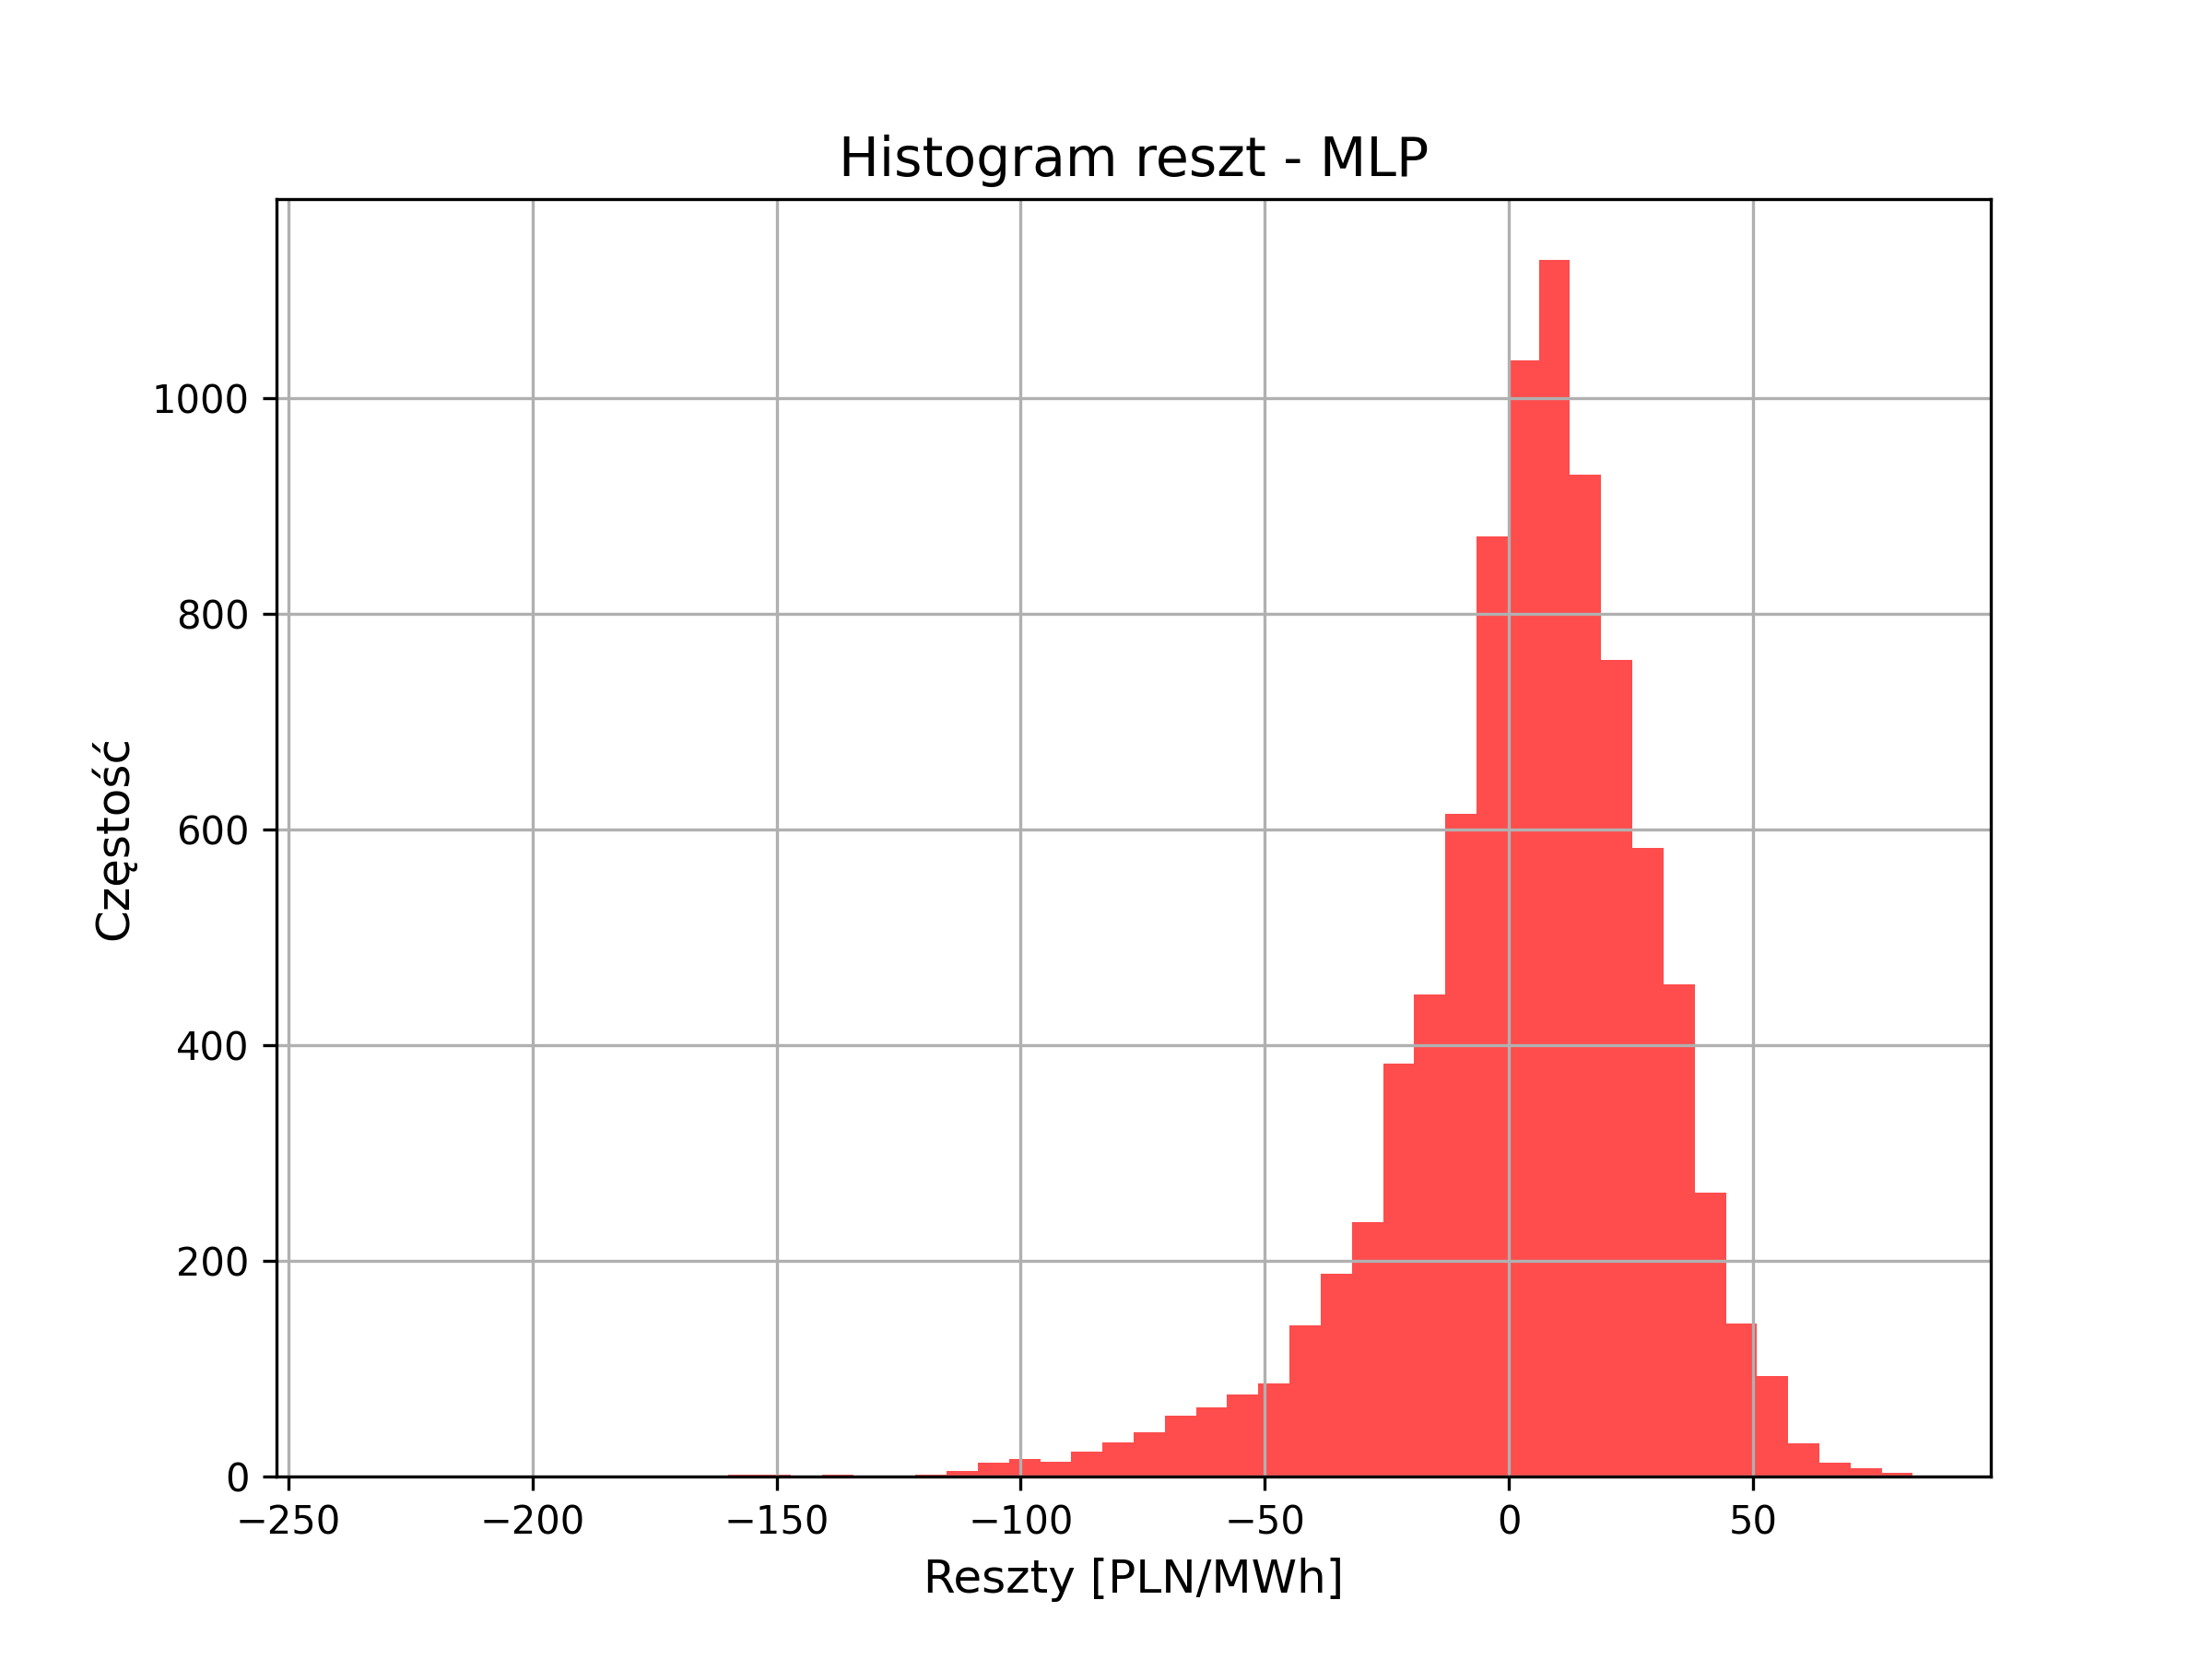
\includegraphics[width=1.0\textwidth]{../../plots/mlp1/mlp_errors_histogram_full_stable_(64, 64, 32, 16, 8).png}
    \caption{Histogram reszt dla modelu MLP w okresie stabilnym. Opracowanie własne.}
    \label{fig:mlp_residuals_stable_period}
\end{figure}

Wykres~\ref{fig:mlp_errors_stable_period} błędów prognoz oscyluje dookoła zera poza okresem w kwietniu, gdzie większość błędów ma wartości ujemne. Widoczne jest, że model MLP ma tendencję do zbyt niskiego oszacowania cen energii elektrycznej w tym okresie. Wartości błędów są znacznie większe niż w przypadku modeli statystycznych, co sugeruje, że model MLP nie radzi sobie dobrze z przewidywaniem cen energii elektrycznej w okresie stabilnym.

Histogram reszt~\ref{fig:mlp_residuals_stable_period} potwierdza te założenia, gdyż mniej przypomina rozkład normalny od poprzednich histogramów. Ma wyższy szczyt, ale jest przesunięty od zera w stronę wartości dodatnich. Większa liczba błędów skupia się w okolicy zera w porównaniu do histogramu reszt dla regresji Ridge lub Prophet.

\section{Okres niestabilny}
\label{sec:okres_niestabilny}

Okres niestabilny obejmuje lata 2020-2023, w których ceny energii elektrycznej były znacznie bardziej zmienne niż w okresie stabilnym. W związku z tym, okres ten może być bardziej wymagający dla modeli prognozujących.

\subsubsection{Regresja liniowa i Ridge}

W analizie wyników regresji liniowej i Ridge dla okresu niestabilnego (2023) dla pełnego i skróconego zbioru danych obserwuje się zbliżone wartości metryk, co wskazuje na ograniczone różnice w skuteczności obu metod w tym okresie. Tabela~\ref{tab:linear_regression_results} przedstawia szczegółowe wyniki dla regresji liniowej i Ridge. Zbiór skrócony podobnie do okresu stabilnego nie przyniósł znaczących różnic w metrykach, ale dodatkowe zmienne w pełnym zbiorze danych lekko poprawiły wyniki niewielkim kosztem obliczeniowym. 

Wysokie wartości MAPE (powyżej 179\%) sugerują problem z wartościami bliskimi zeru ~\ref{subsec:mape}, które pojawiają się w zbiorze danych z okresu niestabilnego. Z tego powodu, MAPE może nie być najlepszą metryką do oceny skuteczności modeli na zbiorze okresu niestabilnego. Z tego powodu większej uwadze poświęcono metrykom MAE, RMSE, sMAPE oraz \(R^2\). Wartości MAE i RMSE są stosunkowo wysokie, co wskazuje na duże błędy prognozowania w jednostkach absolutnych. Błąd na poziomie 59.6 PLN/MWh dla MAE oznacza, że prognozy różnią się średnio o 59.6 PLN od rzeczywistych wartości. Może to prowadzić do znacznych strat finansowych, szczególnie w przypadku dużych transakcji. Wartości sMAPE są dwukrotnie wyższe niż w przypadku okresu stabilnego, co sugeruje, że modele mają trudności z przewidywaniem cen energii w okresach dużej zmienności. Pomimo tego, \(R^2\) nie wzrosło znacząco względem okresu stabilnego, co sugeruje, że modele nadal dobrze wyjaśniają zmienność cen energii, mimo dużych błędów prognozowania. 

Najlepsza wartość hiperparametru \(\alpha\) w regresji Ridge dla okresu niestabilnego wyniosła 0.1, co sugeruje, że w tym przypadku współliniowość między zmiennymi objaśniającymi nie jest tak istotna jak w przypadku pełnego zbioru danych w okresie stabilnym. Wartość ta jest znacznie niższa niż w przypadku pełnego zbioru danych w okresie stabilnym (500.0), co może sugerować, że w okresie niestabilnym modele są bardziej elastyczne.

\begin{table}[H]
    \centering
        \caption{Wyniki metryk dla regresji liniowej i Ridge w okresie niestabilnym (2023). Opracowanie własne.}
        \label{tab:linear_regression_results}
        \begin{tabular}{|l|c|c|c|c|c|}
            \hline
            \textbf{Model} & \textbf{MAE} & \textbf{RMSE} & \textbf{MAPE} & \textbf{sMAPE} & \textbf{\(R^2\)} \\
            \hline
            Regresja liniowa (pełny zbiór) & 59.61 & 77.73 & 179.38 & 16.51 & 0.8111 \\
            Regresja liniowa (skrócony zbiór) & 59.76 & 78.07 & 188.24 & 16.68 & 0.8095 \\
            Regresja Ridge (pełny zbiór) & 59.63 & 77.75 & 179.79 & 16.52 & 0.8110 \\
            Regresja Ridge (skrócony zbiór) & 59.78 & 78.08 & 186.22 & 16.69 & 0.8094 \\
            \hline
        \end{tabular}
\end{table}

Wartości metryk są niemal identyczne dla obu modeli, co sugeruje, że w tym przypadku regularyzacja L2 nie przynosi znaczących korzyści.\newline
Dla dobrego zobrazowania prognoz na wykresie wybrano okres o największej zmienności cen w ramach 2023 roku, czyli od 1 września do 31 października. Wartości prognoz dla regresji Ridge w porównaniu do rzeczywistych cen energii elektrycznej przedstawiono na rysunku~\ref{fig:ridge_predictions_full_sep_oct_2023}. Wykres reszt dla modelu Ridge w okresie niestabilnym przedstawiono na rysunku~\ref{fig:residuals_nonstable_histogram_ridge}.

\begin{figure}[H]
    \centering
    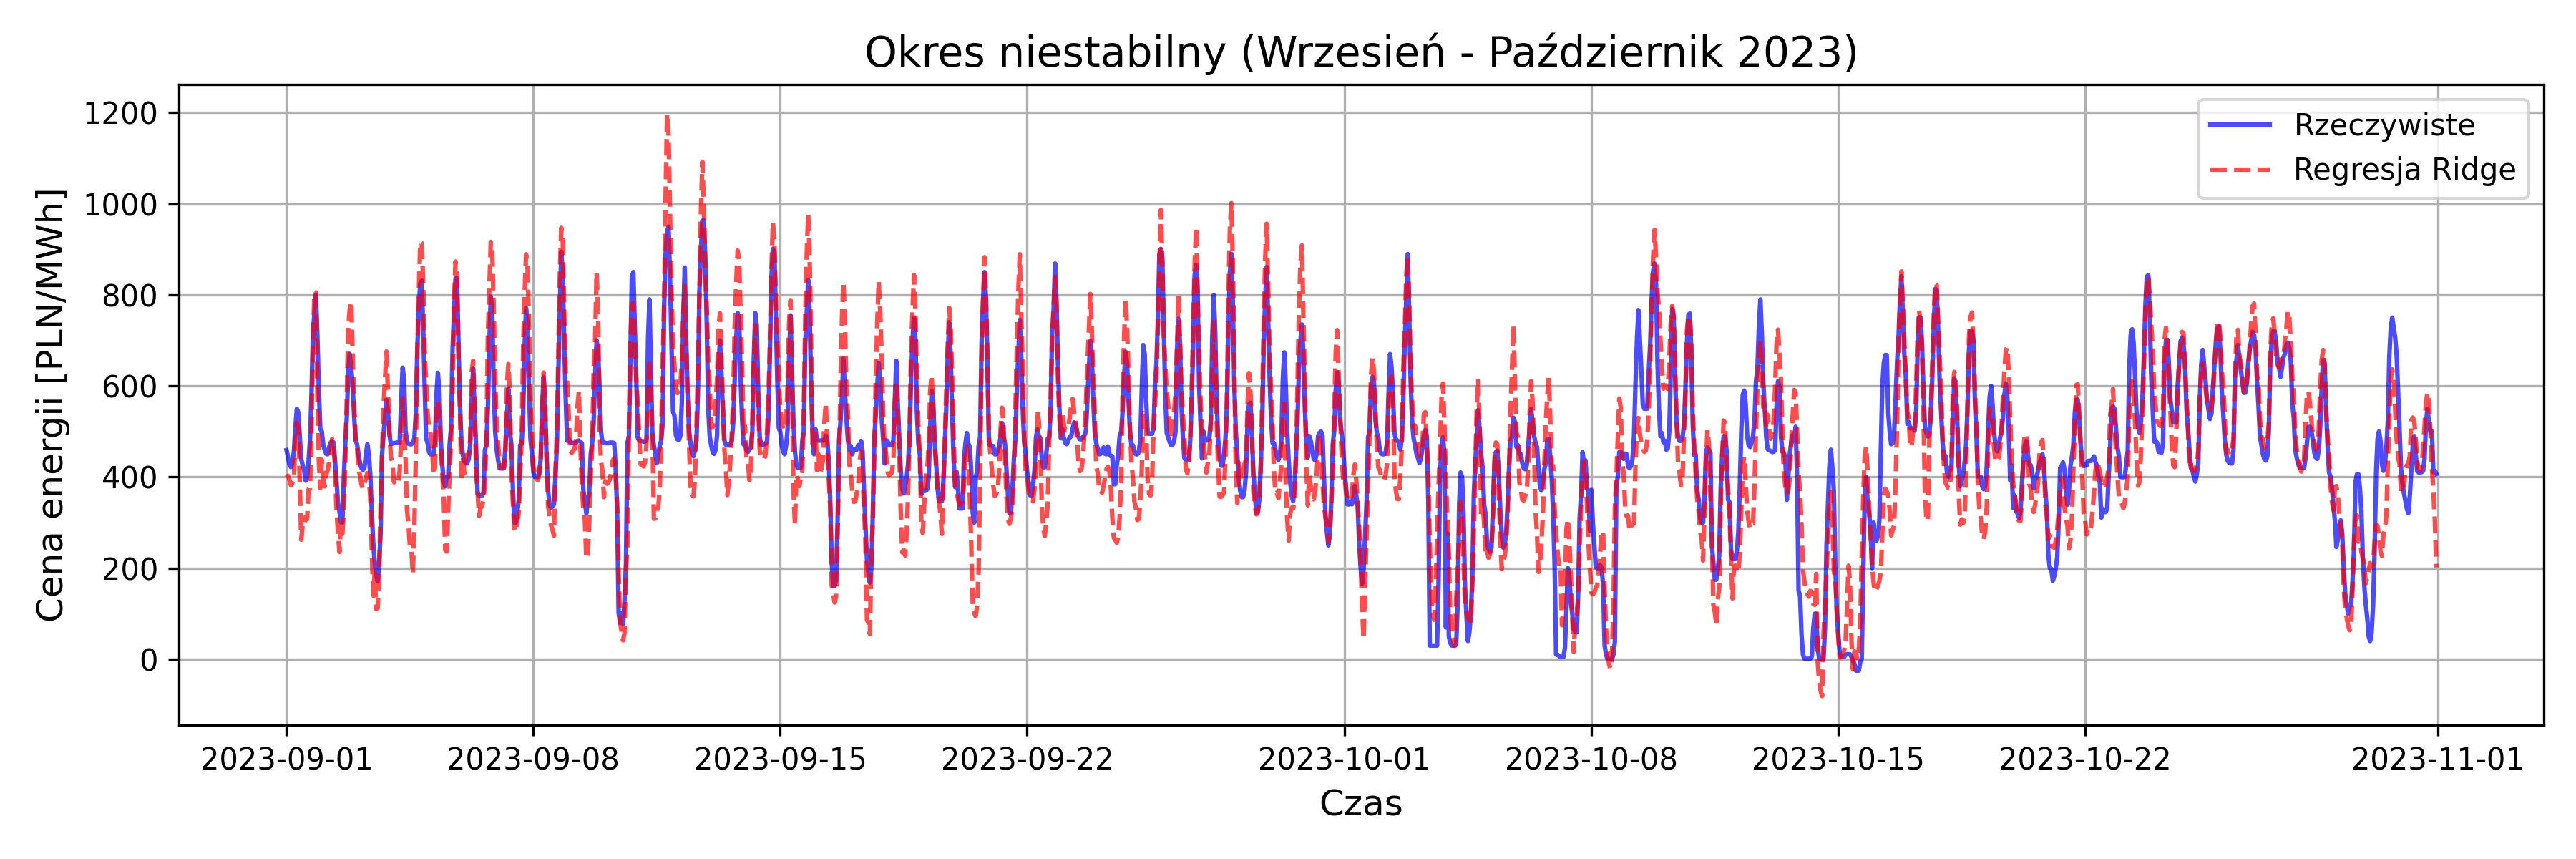
\includegraphics[width=1.0\textwidth]{../../plots/predicts/ridge_predictions_full_sep_oct_2023.png}
    \caption{Prognozy modelu Ridge w porównaniu do rzeczywistych cen energii w okresie niestabilnym (2023). Opracowanie własne.}
    \label{fig:ridge_predictions_full_sep_oct_2023}
\end{figure}

\begin{figure}[H]
    \centering
    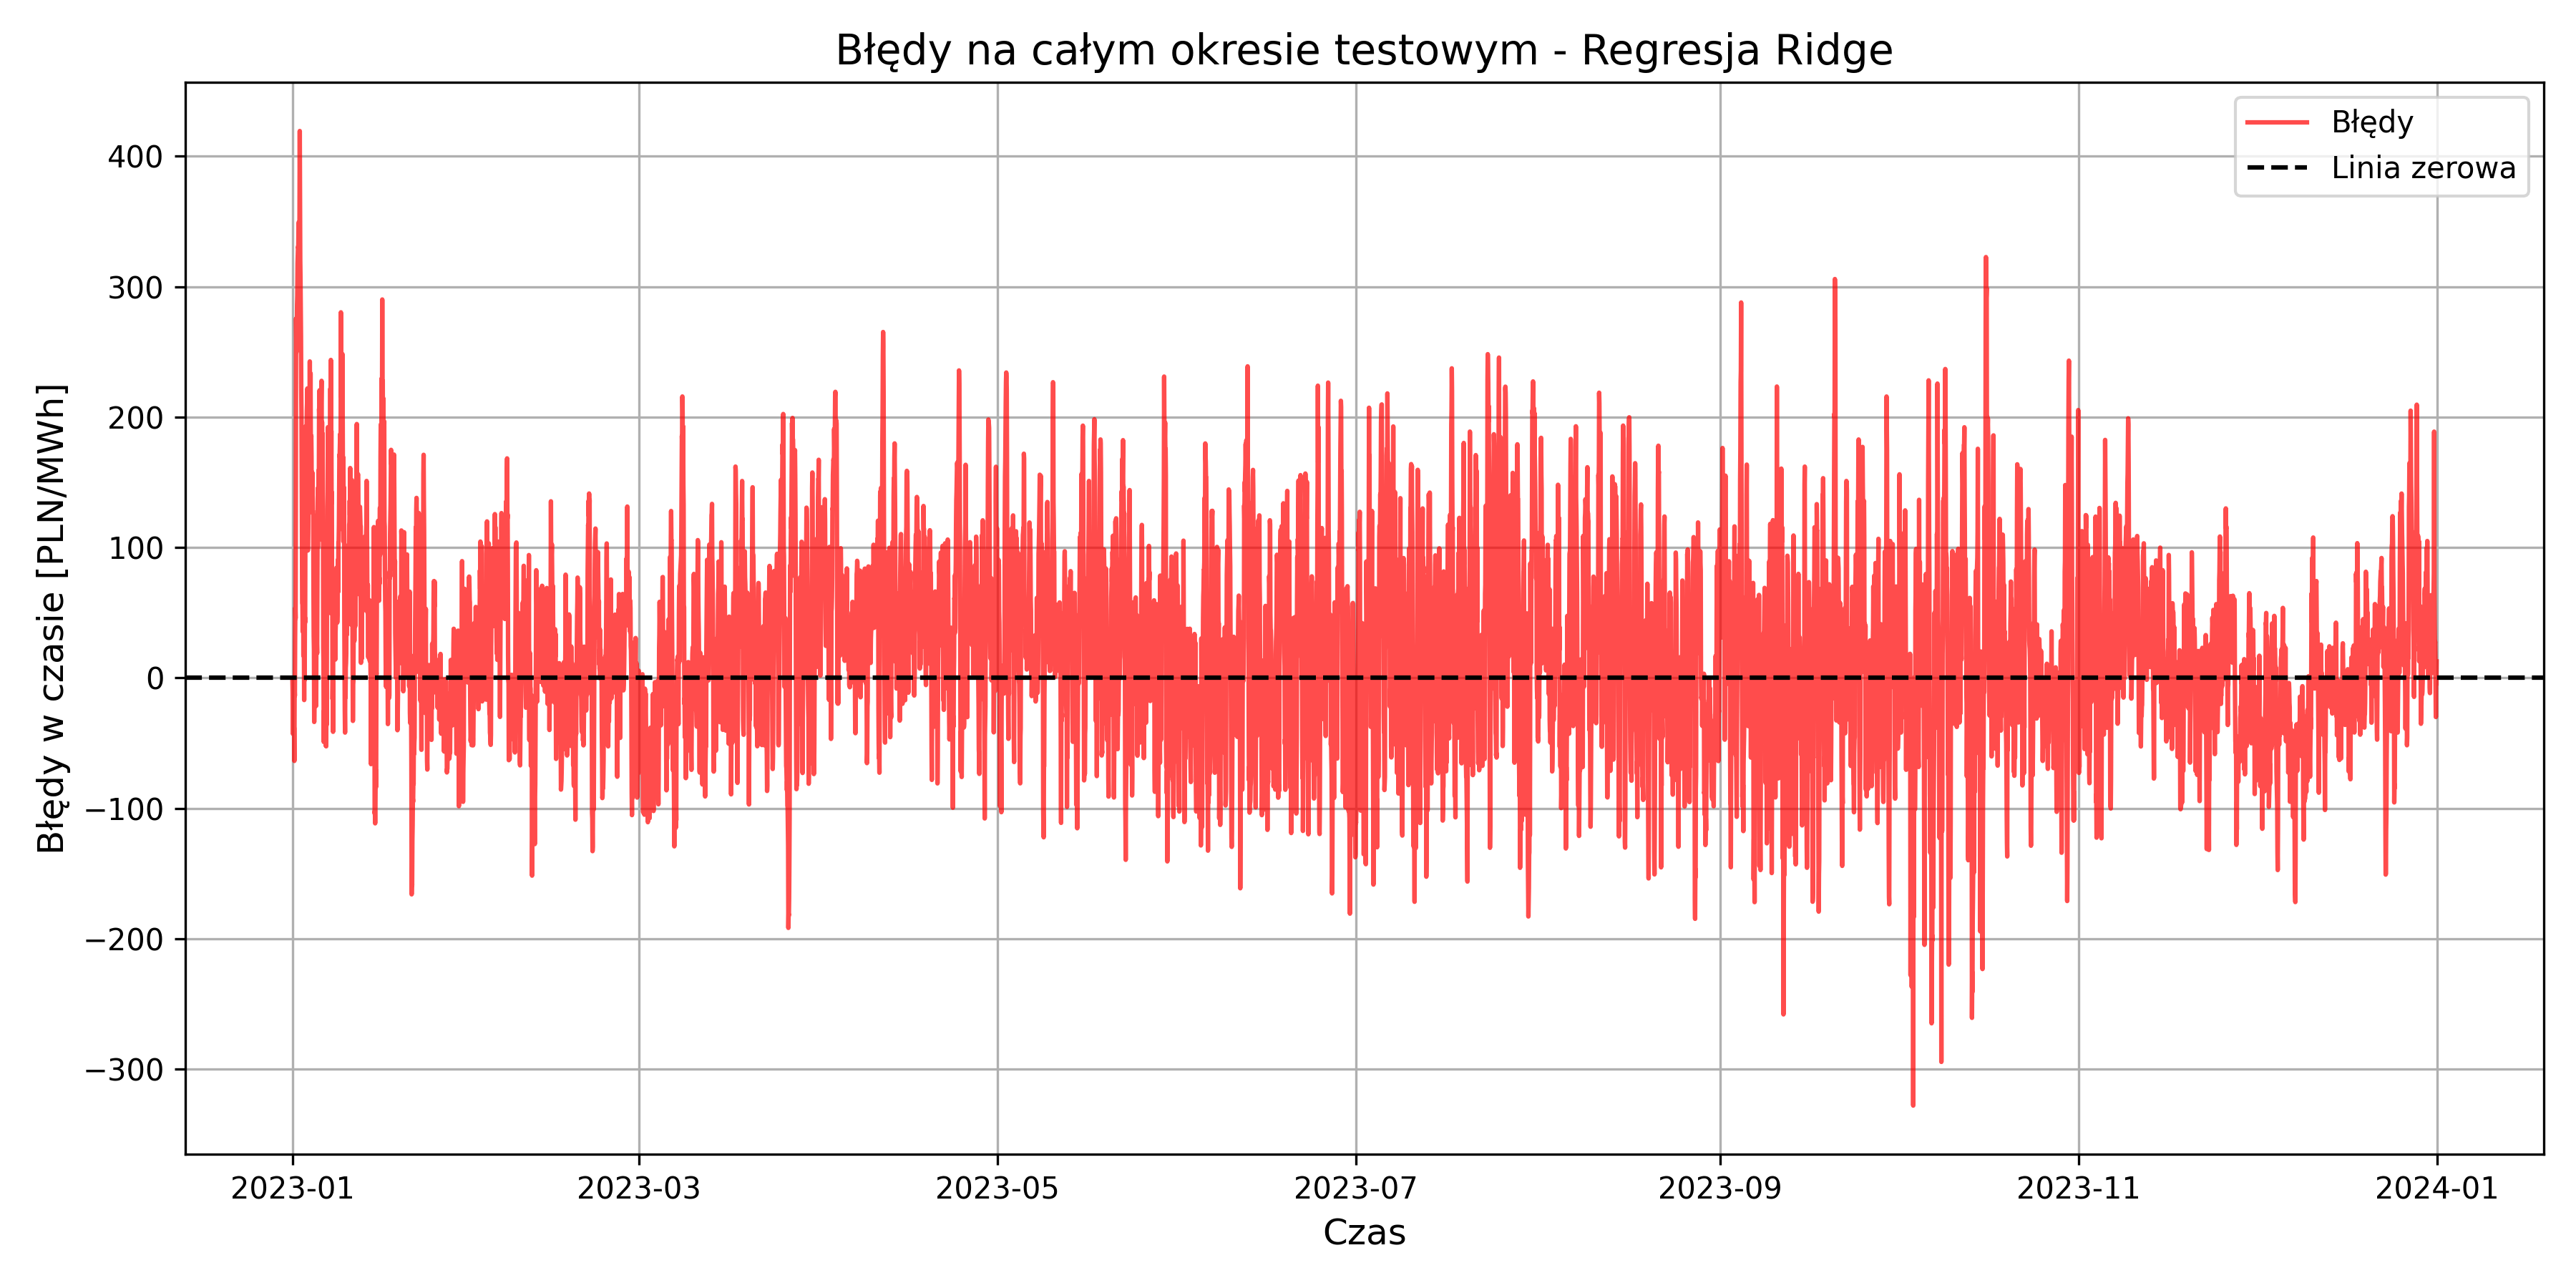
\includegraphics[width=1.0\textwidth]{../../plots/predicts/errors_over_time_Ridge_non_stable_period.png}
    \caption{Błędy prognoz dla modelu Ridge w okresie niestabilnym (2023). Opracowanie własne.}
    \label{fig:ridge_errors_full_sep_oct_2023}
\end{figure}

Na wykresie~\ref{fig:ridge_predictions_full_sep_oct_2023} widać, że model jest skłonny przeszacowywać zmienność cen zarówno w górę, jak i w dół. Błędy prognoz dla modelu Ridge w okresie niestabilnym są znacznie większe niż w przypadku okresu stabilnego. Większość błędów oscyluje się od -100 do 100 PLN/MWh. Największy szczyt można zobaczyć na początku okresu testowego, gdzie obserwuje się szczyt powyżej 400 PLN/MWh. Wartości prognoz są znacznie bardziej rozproszone niż w przypadku okresu stabilnego. Histogram reszt dla modelu Ridge w okresie niestabilnym przedstawiono na rysunku~\ref{fig:residuals_nonstable_histogram_ridge}.

\begin{figure}[H]
    \centering
    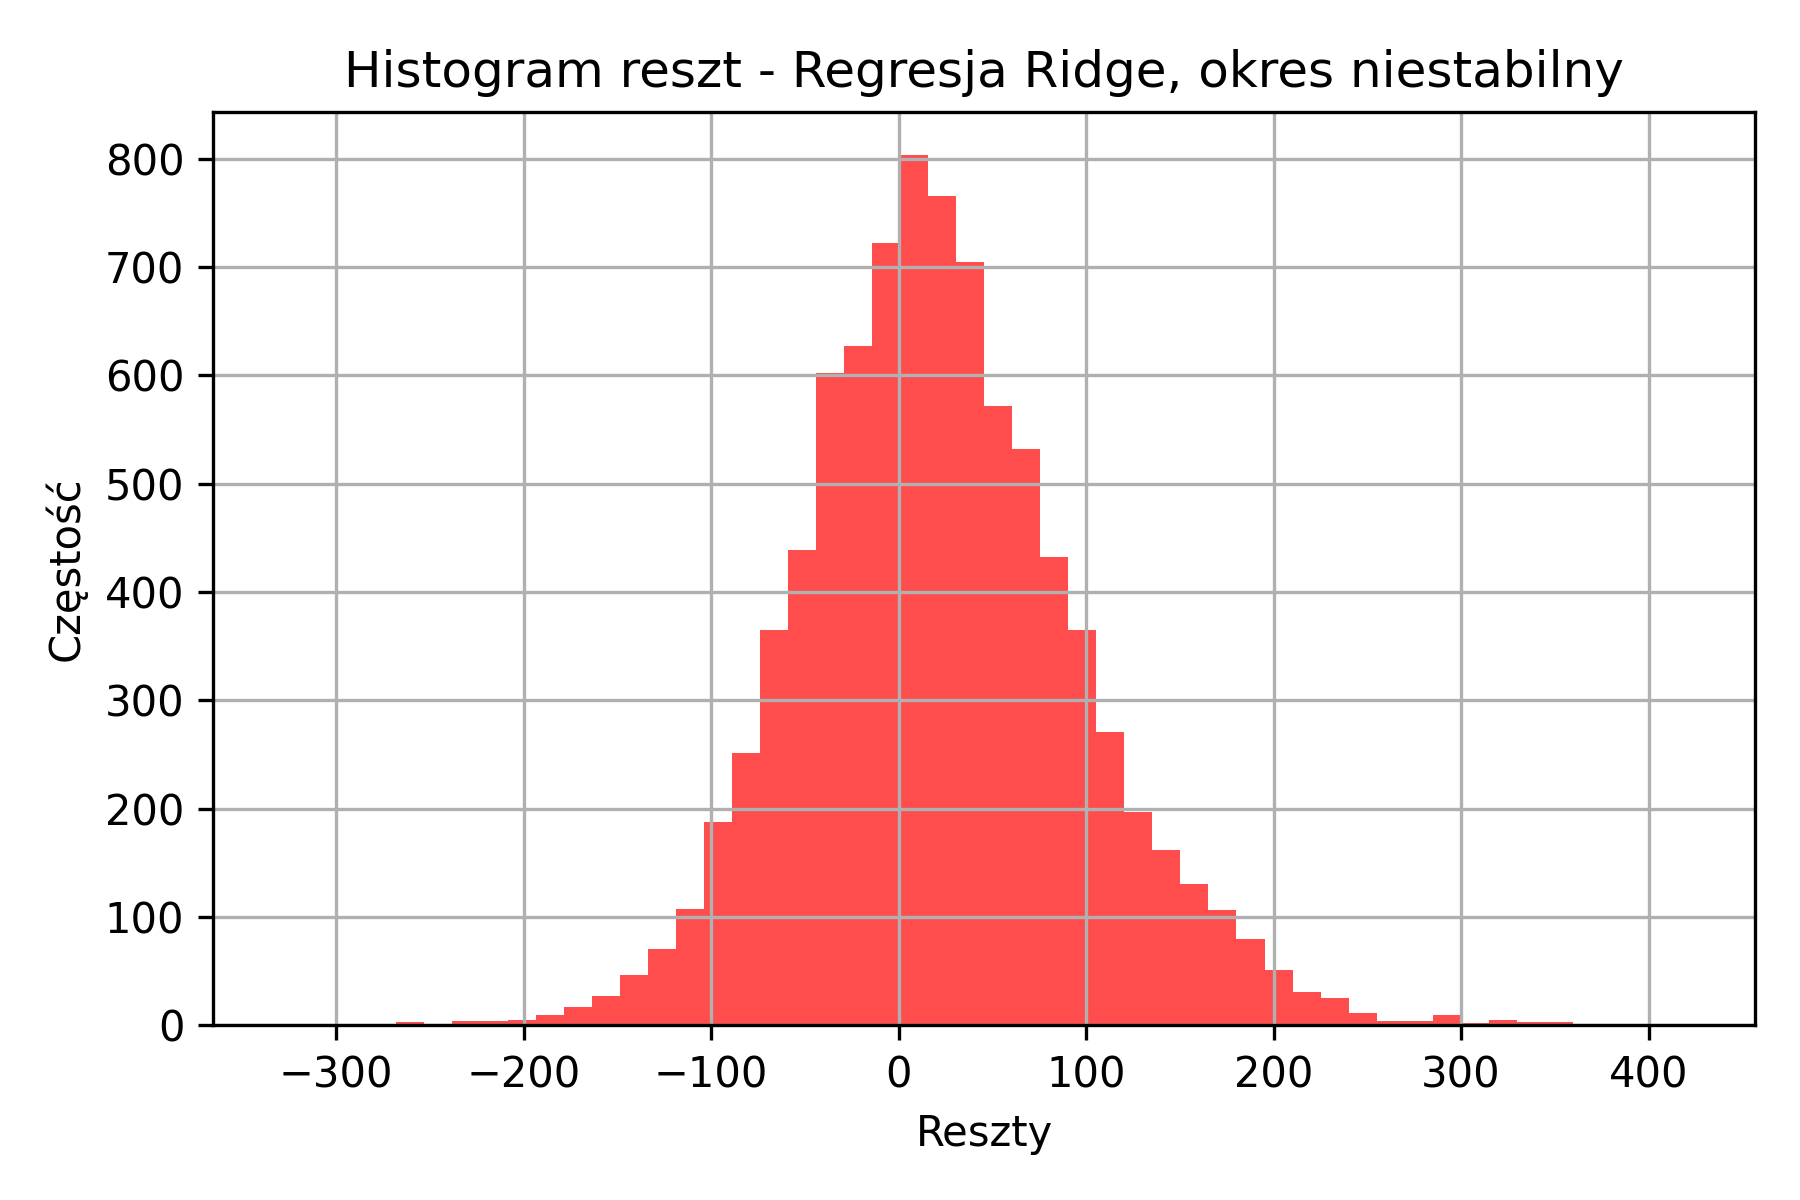
\includegraphics[width=1.0\textwidth]{../../plots/predicts/residuals_histogram_Ridge_not_stable_period.png}
    \caption{Histogram reszt dla modelu Ridge w okresie niestabilnym (2023). Opracowanie własne.}
    \label{fig:residuals_nonstable_histogram_ridge}
\end{figure}

Na podstawie histogramu reszt można zauważyć, że rozkład reszt jest podobny do rozkładu normalnego i ma szczyt w okolicy zera. Porównując histogram reszt z histogramem reszt~\ref{fig:ridge_residuals_stable_period} dla okresu stabilnego, można zauważyć, że histogram reszt w okresie niestabilnym ma szerszy rozkład z większymi ogonami, co potwierdza większe błędy prognozowania w wartościach absolutnych. Histogram reszt jest lekko przesunięty w kierunku wartości dodatnich, co sugeruje, że model ma tendencję do przeszacowywania cen.

\subsubsection{Prophet}

Model Prophet lekko poprawił wyniki w porównaniu do regresji liniowej i Ridge. Najlepszymi parametrami do okresu niestabilnego okazały się (\texttt{changepoint\_prior\_scale=0.001}, \texttt{seasonality\_prior\_scale=50.0}, \texttt{holidays\_prior\_scale=0.1}). Niska wartość {\texttt{changepoint\_prior\_scale}} sugeruje, że model preferuje bardziej stabilne trendy, unikając nadmiernego dopasowania do szumów w danych treningowych. Zwiększona wartość {\texttt{seasonality\_prior\_scale}} pozwala modelowi lepiej uchwycić sezonowe wzorce w danych, co jest istotne w przypadku cen energii elektrycznej, które mogą wykazywać silne sezonowe fluktuacje. Wartość {\texttt{holidays\_prior\_scale}} jest taka sama jak w przypadku okresu stabilnego, co sugeruje, że wpływ świąt na ceny energii wciąż nie jest istotny. Wyniki dla pełnego zbioru danych przedstawiono w tabeli~\ref{tab:prophet_results_combined_nonstable}.

\begin{table}[H]
    \centering
    \caption{Wyniki modelu Prophet dla pełnego i skróconego zbioru danych w okresie niestabilnym (2023).}
    \label{tab:prophet_results_combined_nonstable}
    \begin{tabular}{|l|ccccc|}
        \hline
            \textbf{Zbiór danych} & \textbf{MAE} & \textbf{RMSE} & \textbf{MAPE (\%)} & \textbf{sMAPE (\%)} & \textbf{\(R^2\)} \\
            Pełny     & 57.87 & 74.39 & 163.57 & 16.35 & 0.827021 \\
            Skrócony  & 61.10 & 78.56 & 202.72 & 18.17 & 0.80709 \\
            \hline
    \end{tabular}
\end{table}

Wartość parametru \texttt{changepoint\_prior\_scale} jest najbardziej znacząca w procesie doboru najlepszych hiperparametrów. Zwiększenie wartości tego parametru do 0.1 prowadzi do znacznego pogorszenia wyników na poziomie \textbf{MAE = 138} oraz \textbf{sMAPE = 20.0\%}. Oznacza to, że model zaczyna być bardziej podatny na wykrywanie zmiany w trendzie i próbuje dopasować się do lokalnych fluktuacji. Zmiana innych hiperparametrów zwiększa sMAPE o 1\%.

Wynik modelu prophet w porównaniu z regresją Ridge jest nieznacząco lepszy z punktu widzenia sMAPE, ale średni błąd MAE jest o 1.76 PLN/MWh niższy, co może być bardzo istotne z punktu finansowego w przypadku dużych transakcji. Wartości RMSE są również niższe, co sugeruje, że model Prophet lepiej radzi sobie z przewidywaniem cen energii elektrycznej w okresie niestabilnym.

\begin{figure}[H]
    \centering
    \includegraphics[width=1.0\textwidth]{../../plots/predicts/Prophet_predictions_unstable_sep_pełny_comb_1.png}
    \caption{Porównanie rzeczywistych i przewidywanych wartości cen energii dla modelu Prophet w okresie niestabilnym. Opracowanie własne.}
    \label{fig:prophet_predictions_non_stable_period}
\end{figure}

Wykres predykcji modelu Prophet w okresie niestabilnym jest podobny do wykresu regresji Ridge ~\ref{fig:ridge_predictions_full_sep_oct_2023}. Widać, że model przeszacowuje ceny energii elektrycznej w okresach dużej zmienności, co prowadzi do dużych błędów prognozowania.\newline
Poniżej przedstawiono wykresy błędów prognoz oraz histogram reszt dla modelu Prophet w okresie niestabilnym.

\begin{figure}[H]
    \centering
    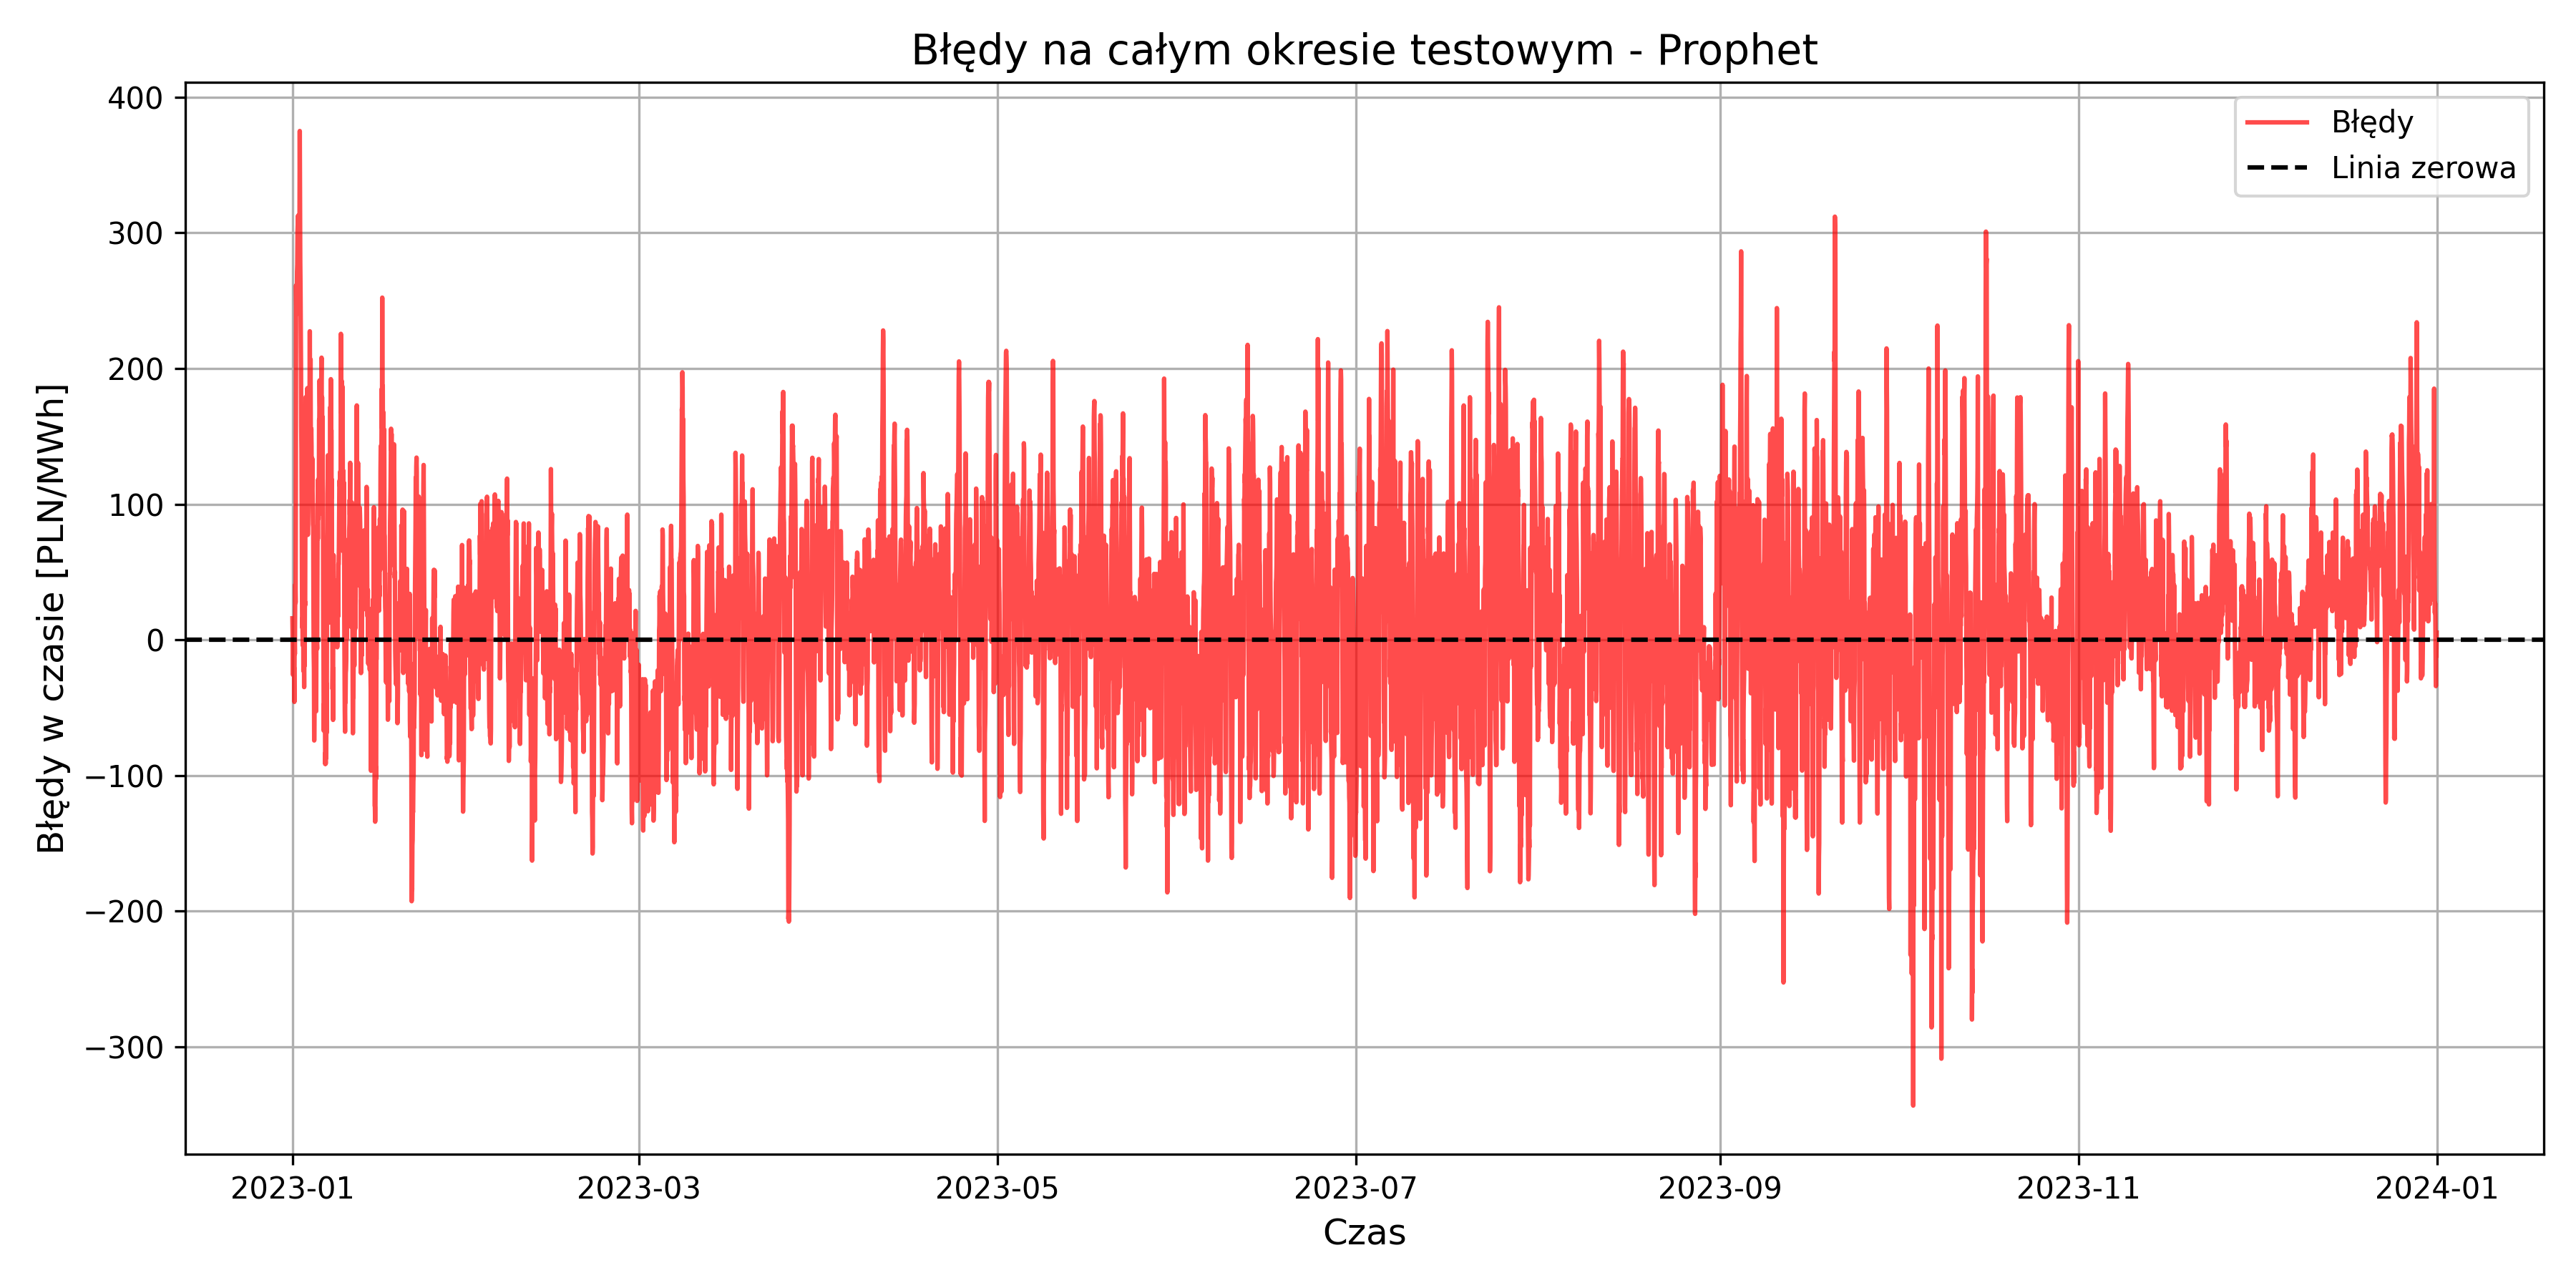
\includegraphics[width=1.0\textwidth]{../../plots/predicts/errors_over_time_Prophet_non_stable.png}
    \caption{Błędy prognoz dla modelu Prophet w okresie niestabilnym. Opracowanie własne.}
    \label{fig:prophet_errors_non_stable_period}
\end{figure}

\begin{figure}[H]
    \centering
    \includegraphics[width=1.0\textwidth]{../../plots/predicts/residuals_histogram_Prophet_unstable_pełny_comb_1.png}
    \caption{Histogram reszt dla modelu Prophet w okresie niestabilnym. Opracowanie własne.}
    \label{fig:prophet_residuals_non_stable}
\end{figure}

Histogram dla modelu Prophet w okresie niestabilnym jest bardziej przesunięty w kierunku wartości dodatnich niż histogram dla regresji Ridge~\ref{fig:residuals_nonstable_histogram_ridge}. Histogram wykazuje większe odchylenia od rozkładu normalnego, i nie posiada szczytu w zerze. Natomiast ogon histogramu po prawej stronie jest krótszy. To jest prawdopodobnie powodem, że model Prophet ma lepsze wyniki od regresji Ridge. 

\subsubsection{MLP}

Dla uzyskania najlepszych wyników dla modelu MLP w okresie niestabilnym, liczbę epok zwiększono do 1000, a rozmiar partii zmniejszono do 64. Wartości hiperparametrów pozostały takie same jak w przypadku okresu stabilnego. Szybkość uczenia została zwiększona do 0.001, co pozwoliło na szybsze dostosowywanie wag. Po raz pierwszy wyniki skróconego zestawu parametrów przewyższyły wyniki pełnego zbioru danych we wszystkich metrykach. Sugeruje to, że model MLP jest bardziej podatny na nadmierne dopasowanie do danych treningowych w przypadku pełnego zbioru danych.\newline
Wartości metryk dla pełnego i skróconego zbioru danych przedstawiono w tabeli~\ref{tab:mlp_results_combined_nonstable}.

\begin{table}[H]
    \centering
    \caption{Wyniki modelu MLP dla pełnego i skróconego zbioru danych w okresie niestabilnym (2023).}
    \label{tab:mlp_results_combined_nonstable}
    \begin{tabular}{|l|cccccc|}
        \hline
        \textbf{Zbiór danych} & \textbf{MAE} & \textbf{RMSE} & \textbf{MAPE (\%)} & \textbf{sMAPE (\%)} & \textbf{\(R^2\)} \\
        Pełny     & 98.85 & 126.89 & 1361.22 & 22.21 & 0.50 \\
        Skrócony  & 66.08 & 88.46 & 1702.13 & 17.38 & 0.76 \\
        \hline
    \end{tabular}
\end{table}

Skrócony zestaw parametrów wyjaśnił 76\% zmienności cen energii elektrycznej, co jest znacznie lepszym wynikiem niż w przypadku pełnego zbioru danych. Jest to jednak wciąż gorszy wynik niż w przypadku wcześniejszych modeli. Wartości absolutne MAE i sMAPE są przykładowo o 8.21 PLN/MWh i 1.03\% gorsze niż w przypadku modelu Prophet.\newline
Wykres rzeczywistych i przewidywanych wartości dla modelu MLP w okresie niestabilnym dla danych skróconych przedstawiono na rysunku~\ref{fig:mlp_predictions_non_stable_period}.

\begin{figure}[H]
    \centering
    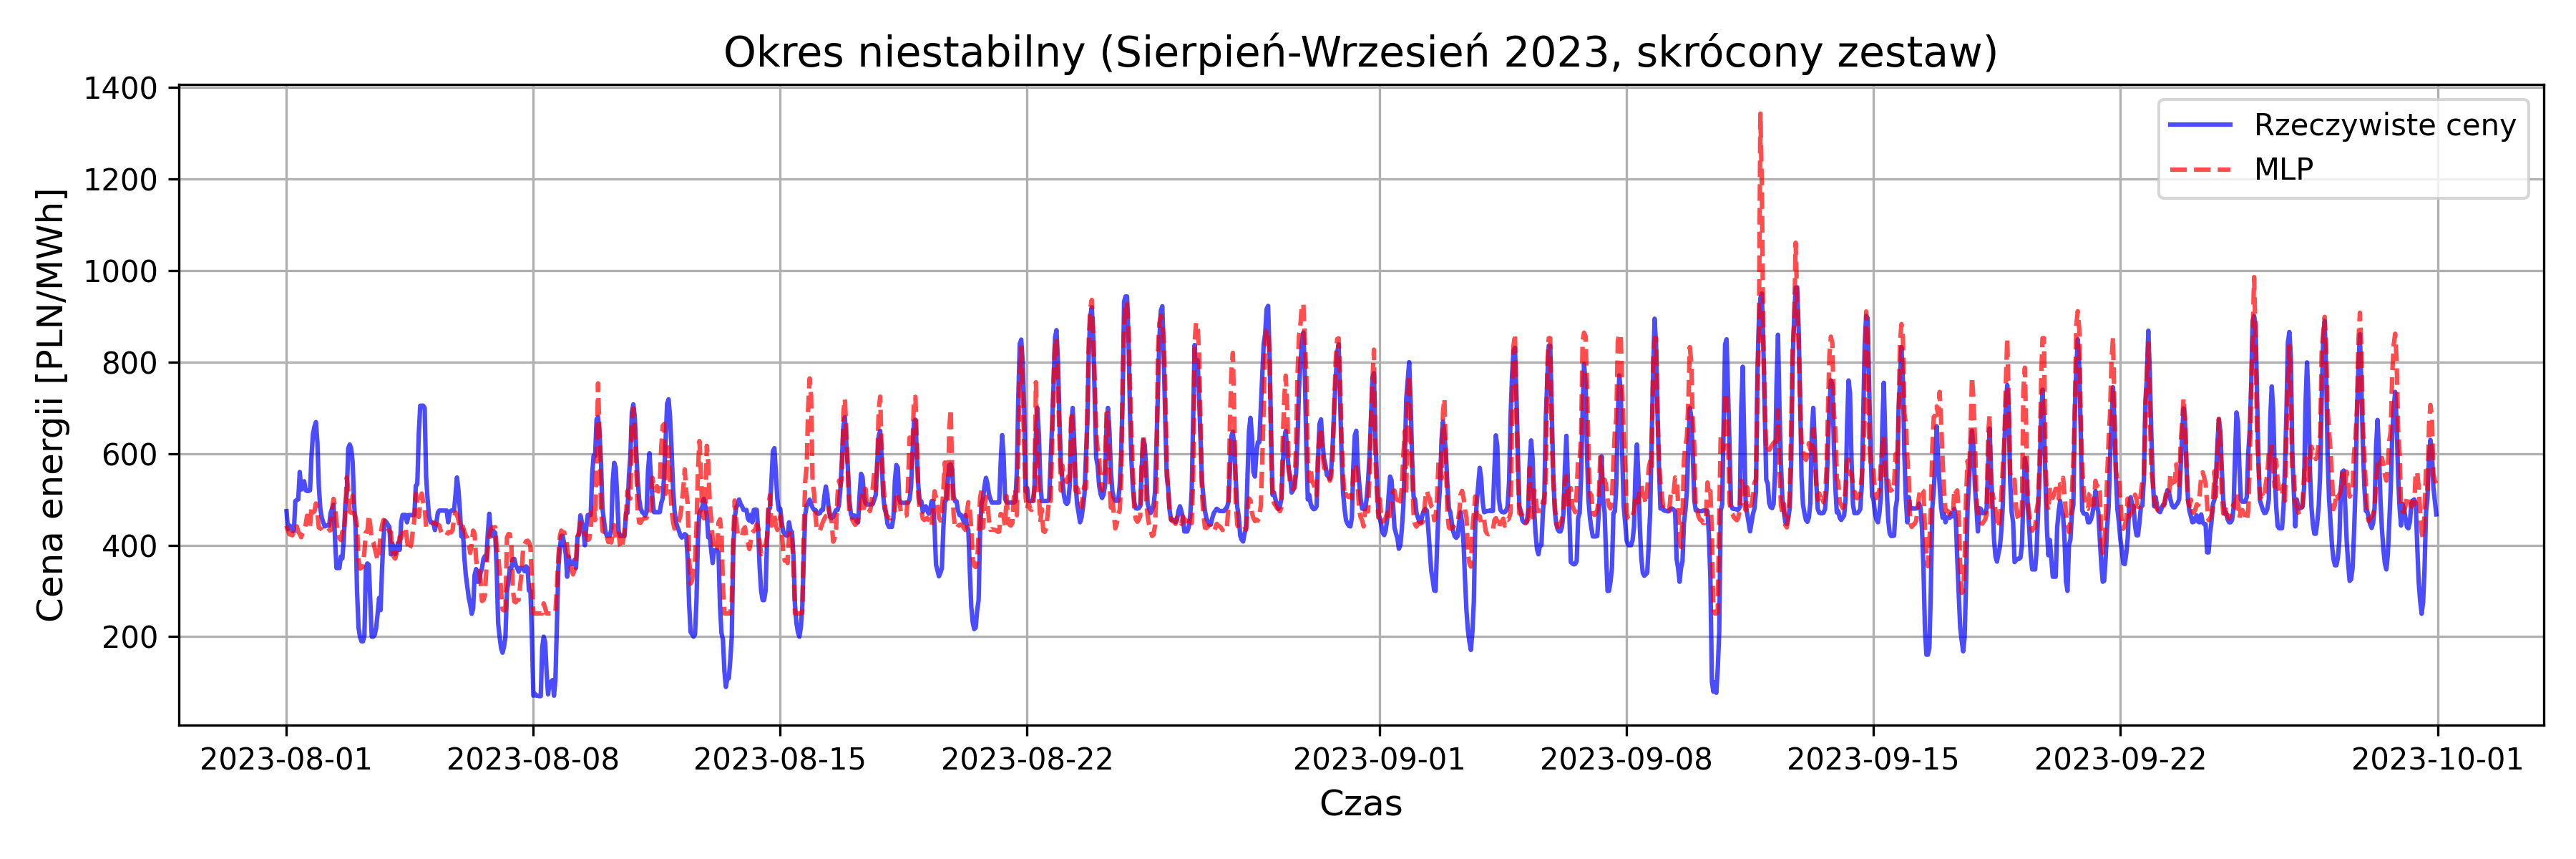
\includegraphics[width=1.0\textwidth]{../../plots/mlp2/mlp_predictions_short_unstable_aug_sep_(64, 64, 32, 16, 8).png}
    \caption{Porównanie rzeczywistych i przewidywanych wartości cen energii dla modelu MLP w okresie niestabilnym. Opracowanie własne.}
    \label{fig:mlp_predictions_non_stable_period}
\end{figure}

Wykres potwierdza gorsze wyniki modelu MLP w porównaniu do modelu Prophet. Prawie wszystkie szczyty oscylacji cenowej są przeszacowane, a model MLP nie jest w stanie dokładnie przewidzieć poziomu wzrostów ani spadków cen energii elektrycznej. Wartości prognoz są znacznie bardziej rozproszone niż w przypadku modelu Prophet.

\begin{figure}[H]
    \centering
    \includegraphics[width=1.0\textwidth]{../../plots/mlp2/errors_over_time_(64, 64, 32, 16, 8)_Niestabilny_2023_skrócony.png}
    \caption{Błędy prognoz dla modelu MLP w okresie niestabilnym. Opracowanie własne.}
    \label{fig:mlp_errors_non_stable_period}
\end{figure}

Wykres błędów prognoz dla modelu MLP w okresie niestabilnym~\ref{fig:mlp_errors_non_stable_period} również potwierdza gorsze wyniki modelu MLP. Wartości absolutne błędów dochodzą do poziomu 400 PLN/MWh.

Histogram reszt~\ref{fig:mlp_residuals_non_stable_period} dla modelu MLP ma szczyt w okolicy zera, ale ma dłuższe ogony po obu stronach. Histogram wykazuje większe odchylenia od rozkładu normalnego. Widoczne są reszty o dużych wartościach, szczególnie po lewej stronie histogramu.

\begin{figure}[H]
    \centering
    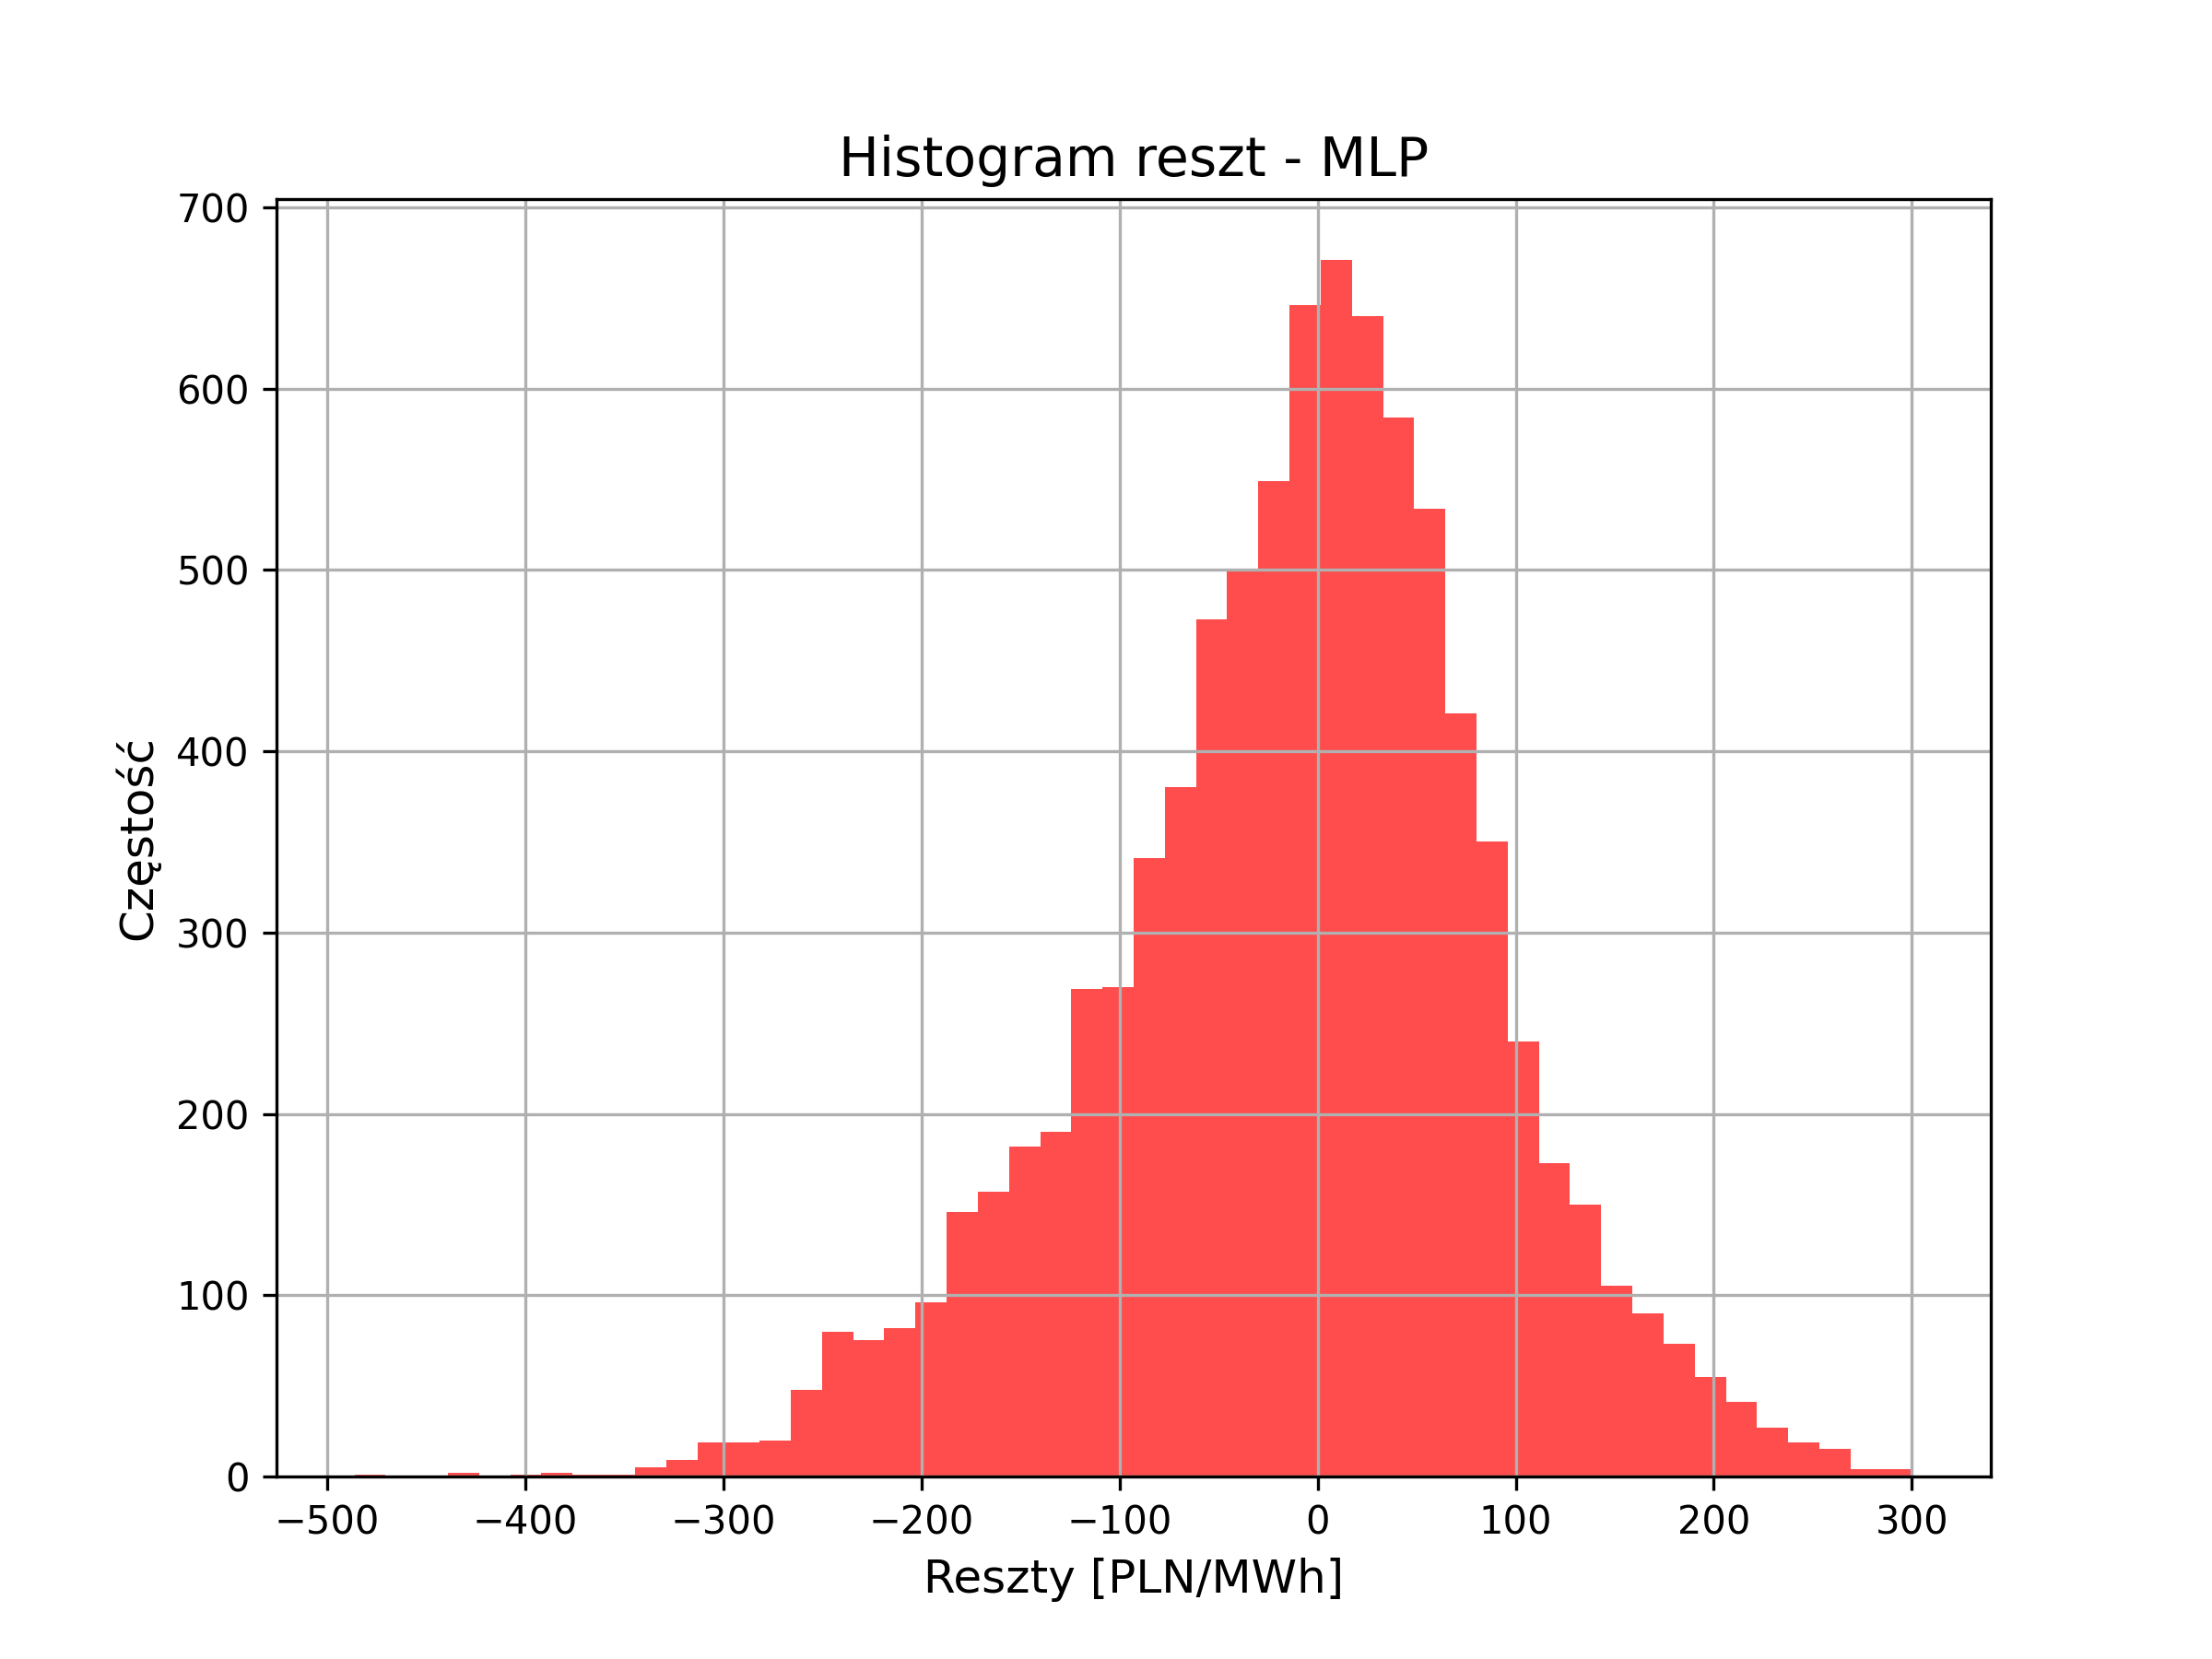
\includegraphics[width=1.0\textwidth]{../../plots/mlp2/mlp_errors_histogram_short_unstable_(64, 64, 32, 16, 8).png}
    \caption{Histogram reszt dla modelu MLP w okresie niestabilnym. Opracowanie własne.}
    \label{fig:mlp_residuals_non_stable_period}
\end{figure}
